\documentclass[12pt, aspectratio = 169]{beamer}
\usepackage[T2A]{fontenc}
\usepackage[utf8]{inputenc}
\usepackage[russian,english]{babel}
\usepackage{animate} %for gifs
\usepackage{graphicx} %for gifs
\usepackage{array}
\usepackage{amssymb,amsfonts,amsmath,mathtext, bm,mathtools}
\usepackage{cite,enumerate,float,indentfirst}

\usepackage{cancel}
%\usepackage{hepunits}
%\usepackage{physics}
\usepackage{subfigure}
\usepackage{xcolor}
\usepackage{relsize}

\usepackage{tikz}
\usepackage{marvosym} %arrows
\usepackage{ulem} %  for text strikeout

\usetikzlibrary{positioning,shapes,arrows}

\graphicspath{{images/}}
\definecolor{calmRed}{rgb}{0.82, 0.1, 0.26}
\definecolor{calmBlue}{rgb}{0.15, 0.23, 0.89} %palantinblue
\definecolor{calmGreen}{rgb}{0.0, 0.65, 0.31}
\definecolor{DESYBlue}{RGB}{0,139,213}
\definecolor{calmYellow}{rgb}{0.9, 0.6, 0}

\newcommand{\red}{\color{calmRed}}
\newcommand{\blue}{\color{calmBlue}}
\newcommand{\green}{\color{calmGreen}}
\newcommand{\yellow}{\color{calmYellow}}
\newcommand{\black}{\color{black}}

\usetheme{Madrid}
\usecolortheme[RGB={0,139,213}]{structure}
\setbeamertemplate{itemize items}[circle]
\setbeamertemplate{enumerate items}[circle]

\setbeamercolor{footline}{fg=DESYBlue}
\setbeamercolor{section in head/foot}{fg=white, bg=black}

\newcommand{\backupbegin}{
	\newcounter{finalframe}
	\setcounter{finalframe}{\value{framenumber}}
}
\newcommand{\backupend}{
	\setcounter{framenumber}{\value{finalframe}}
}
\beamertemplatenavigationsymbolsempty

\setbeamertemplate{navigation symbols}[nodate]{} 
\title{Artificial neural networks}
\author[name]{Olga Razuvaeva\inst{1, 2}, Sergey Korpachev\inst{3, 4} and Stepan Zakharov \inst{5}}%
\institute{
	\inst{1} Institute for Theoretical and Experimental Physics
	\newline
	\inst{2} National Research Nuclear University MEPhI (Moscow Engineering Physics Institute)
	\newline
	\inst{3} Moscow Institute of Physics and Technology
	\newline
	\inst{4} Lebedev Physical Institute of the Russian Academy of Sciences
	\newline
	\inst{5} Novosibirsk State University
	\newline
	\vspace{1em}

	
\includegraphics[width=2.0cm]{itep_logo.png}\hspace*{0.5cm}
	
\includegraphics[width=2.0cm]{mephi_logo.jpg}\hspace*{0.1cm}
	
\includegraphics[width=3.5cm]{mipt_logo.png}\hspace*{0.1cm}
	
\includegraphics[width=2.0cm]{lpi_logo.png}\hspace*{0.6cm}
	
\includegraphics[width=3.5cm]{nsu_logo.png}\hspace*{0.3cm}
}

\date{}

\begin{document}
	\setbeamertemplate{footline}{}
	\maketitle
	\setbeamertemplate{footline}{
		\leavevmode%
		\hbox{%
			\begin{beamercolorbox}[wd=.4\paperwidth,ht=2.25ex,dp=1ex,center]{}%
				Olga Razuvaeva, ITEP and MEPhI, Moscow, Russia
			\end{beamercolorbox}%
			\begin{beamercolorbox}[wd=.3\paperwidth,ht=2.25ex,dp=1ex,center]{}%
				November 22, 2020
			\end{beamercolorbox}%
			\begin{beamercolorbox}[wd=.3\paperwidth,ht=2.25ex,dp=1ex,right]{}%
				Slide \insertframenumber{} / \inserttotalframenumber \hspace*{2ex}
		\end{beamercolorbox}}
	}

%----------------------------------------------------------------------

\begin{frame}
    \frametitle{Outline}
    \begin{itemize}
    	\centering
    	\item Non-linearity in data
    	\item Feature extraction
    	\item ANN structure
	    \item How to train?
	    \item Evolution of GD
	    \item Deep Learning
	    \item The Achilles heel of the DL models
	    \item Reaching stability
	    \item Network architectures
    \end{itemize}
\end{frame}

%----------------------------------------------------------------------

\begin{frame}
	\frametitle{Non-linearity in data}
	\centering
	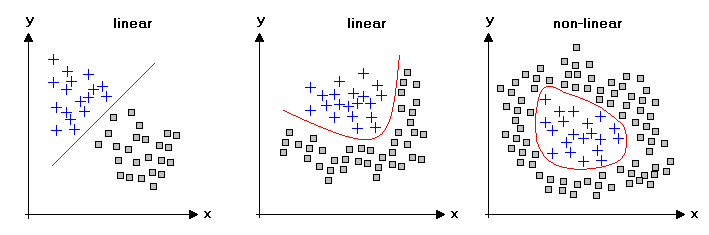
\includegraphics[width=1\linewidth]{lin_nonlin.png}
	Do you know how to describe the non-linear data in the right picture?\\
	Linear model, seriously?\\
	\href{http://www.statistics4u.com/fundstat_eng/cc_linvsnonlin.html}{\color{blue}\uline{Source}}\\
	\href{https://blog.minitab.com/blog/adventures-in-statistics-2/what-is-the-difference-between-linear-and-nonlinear-equations-in-regression-analysis}{\color{blue}\uline{Other link}}
\end{frame}

%----------------------------------------------------------------------

\begin{frame}
	\frametitle{Feature extraction}
	\begin{columns}[T]
	    \column{0.4\textwidth}
	    \begin{minipage}[t]{\linewidth}
            \begin{itemize}
            \item Consider some simpler data
	        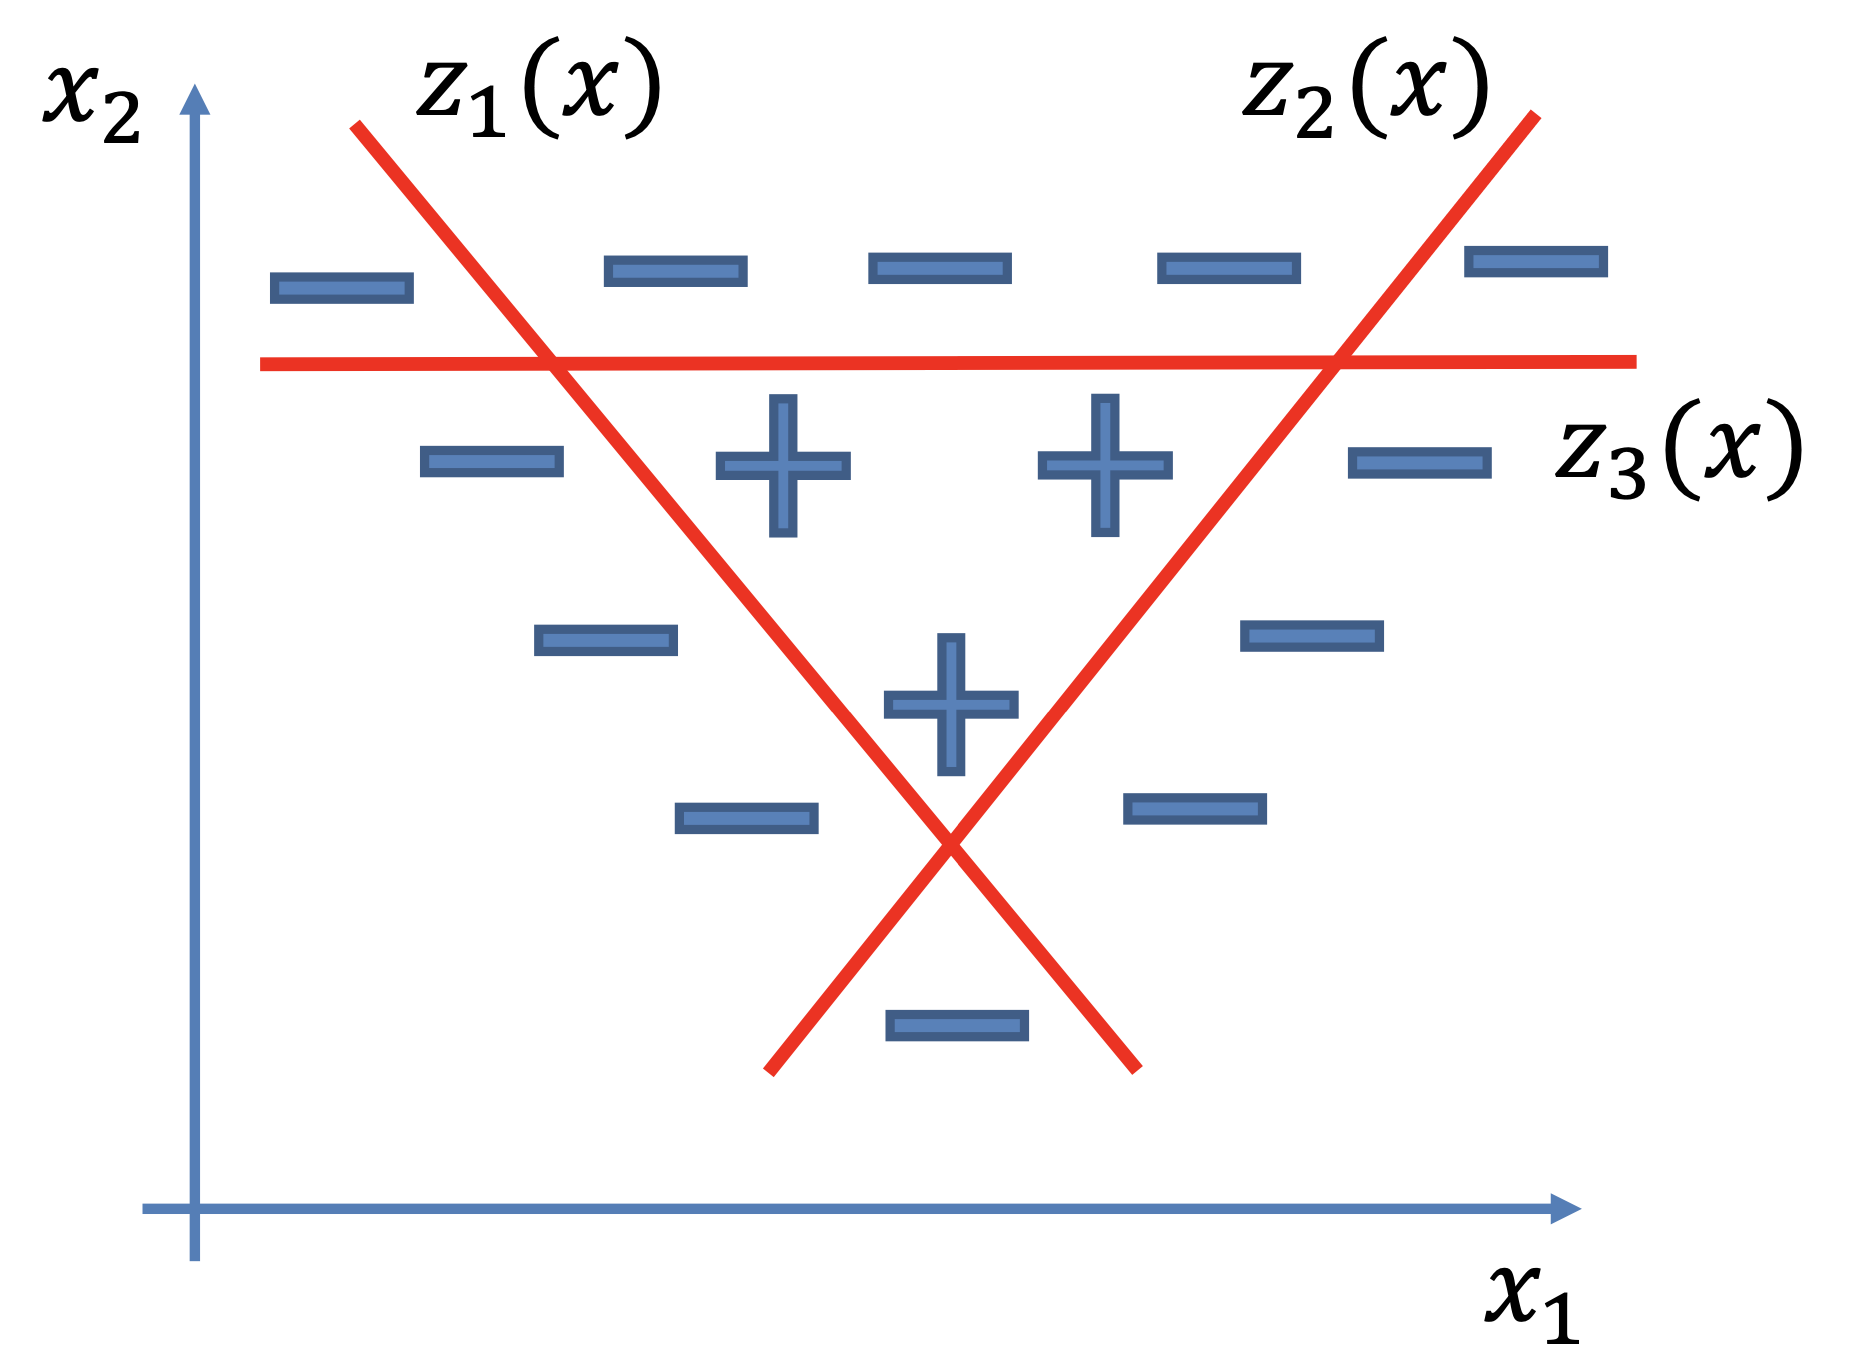
\includegraphics[width=0.7\linewidth]{triangle.png}
            \item \onslide<2->{Let's try to describe it with \\ 
            a linear model 
            $z_i(\bm x) = \bm \omega_0,_i + \bm \omega_1,_i \cdot \bm x_1 + \bm \omega_2,_i \cdot \bm x_2$}
            \end{itemize}
        \end{minipage}
		\column{0.6\textwidth}
    	\begin{minipage}[t]{\linewidth}
            \begin{itemize}
                \onslide<3->{\item Let's rewrite new variables $z_i(\bm x)$ in the form of a computational graph
                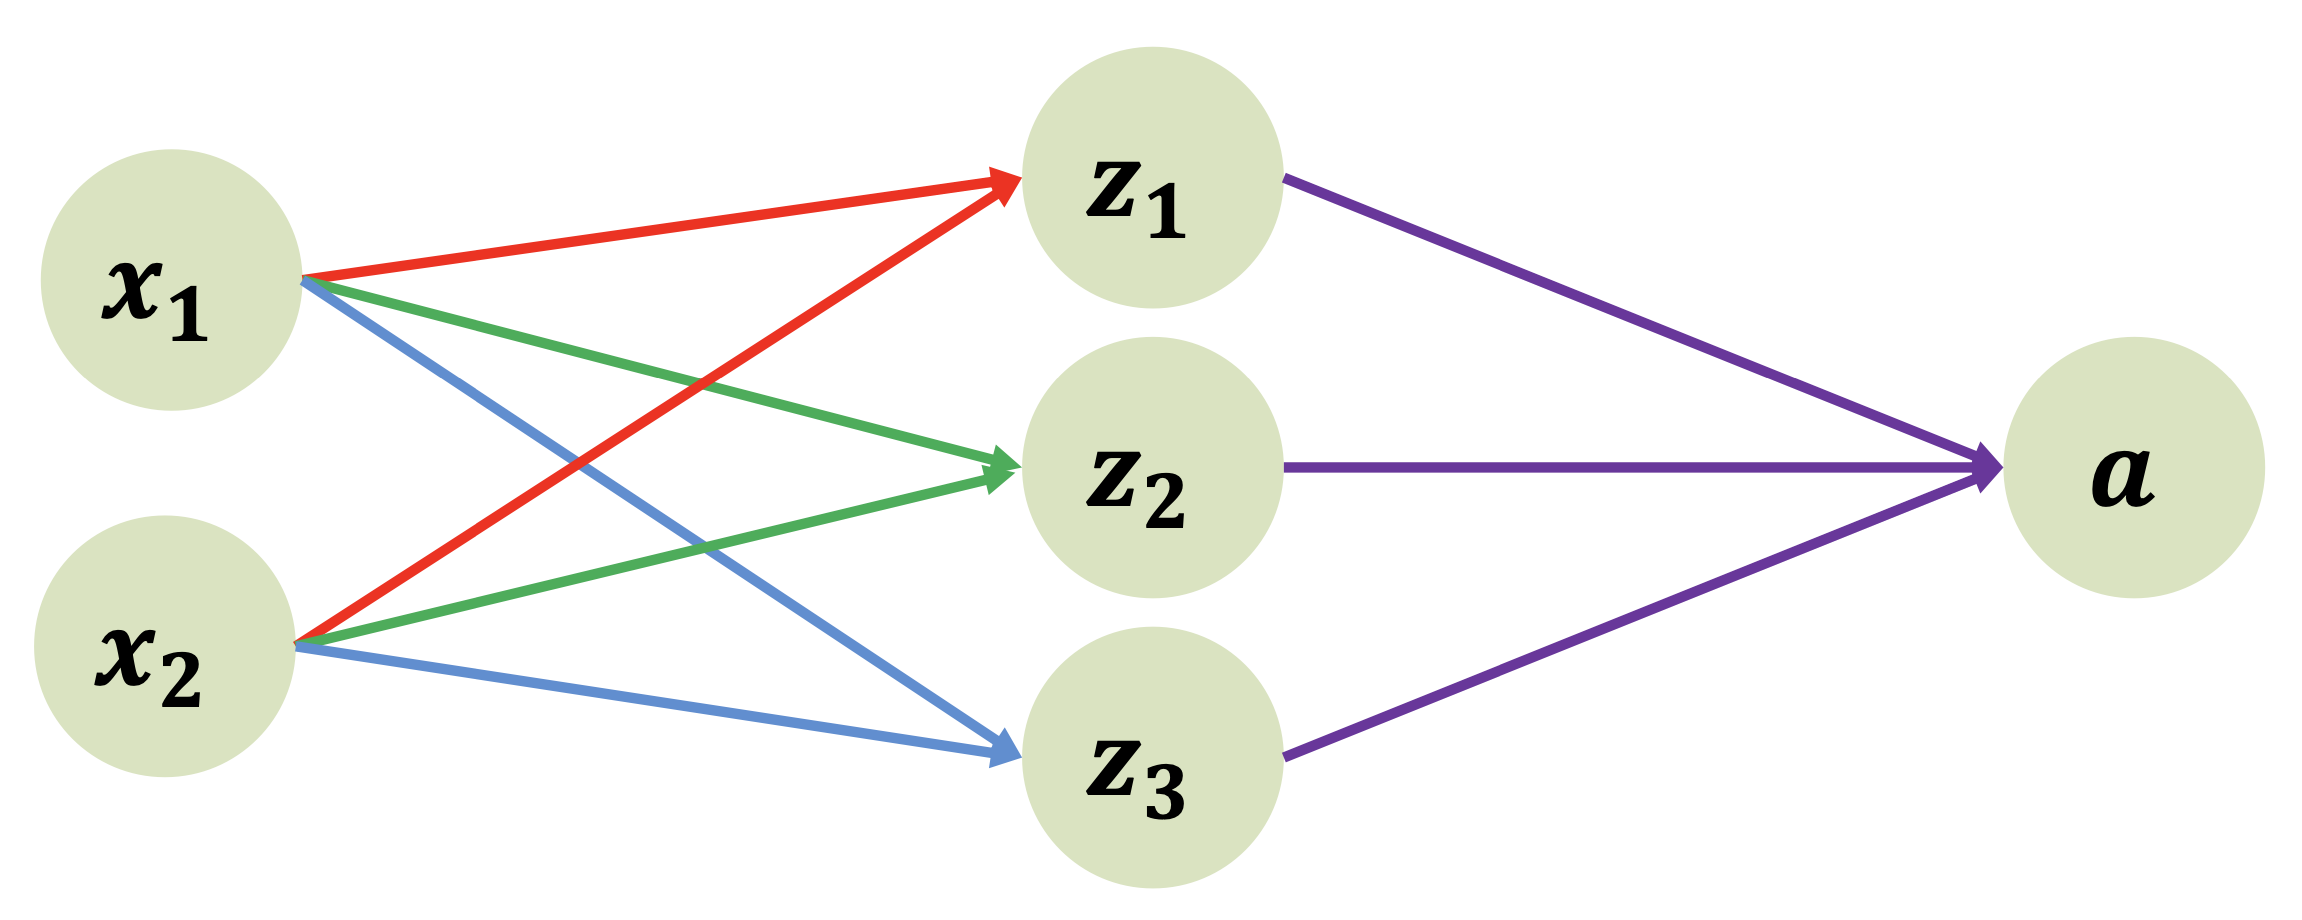
\includegraphics[width=0.7\linewidth]{graph.png}}
            \end{itemize}
            \begin{itemize}
                \onslide<4->{\item Now our model is:\\
                $a(\bm x) = \bm k_0 + \bm k_1 \cdot (\bm \omega_0,_1 + \bm \omega_1,_1 \cdot \bm x_1 + \bm \omega_2,_1 \cdot \bm x_2) + \bm k_2 \cdot (\bm \omega_0,_2 + \bm \omega_1,_2 \cdot \bm x_1 + \bm \omega_2,_2 \cdot \bm x_2) + \bm k_3 \cdot (\bm \omega_0,_3 + \bm \omega_1,_3 \cdot \bm x_1 + \bm \omega_2,_3 \cdot \bm x_2)$}
                \onslide<5->{\item The model is linear, how to create new features?}
            \end{itemize}
        \end{minipage}
    \end{columns}
    \centering
    \hfill \break
    \onslide<1->{
    \href{https://www.coursera.org/learn/intro-to-deep-learning/lecture/yy1NV/multilayer-perceptron-mlp}{\color{blue}\uline{Source}}}
\end{frame}

%----------------------------------------------------------------------

\begin{frame}
    \frametitle{Computation graph}
	\begin{columns}[T]
	    \column{0.5\textwidth}
	    \begin{minipage}[t]{\linewidth}
            \begin{itemize}
            \item Add non-linearity to our model to create new features
            \item \onslide<2->{Now we have:
            $a(\bm x) = \red \bm\sigma \black \big(\bm k_0 + \bm k_1 * \red \bm\sigma \black(\bm \omega_0,_1 + \bm \omega_1,_1 * \bm x_1 + \bm \omega_2,_1 * \bm x_2) + \bm k_2 * \red \bm\sigma \black(\bm \omega_0,_2 + \bm \omega_1,_2 * \bm x_1 + \bm \omega_2,_2 * \bm x_2) + \bm k_3 * \red \bm\sigma \black(\bm \omega_0,_3 + \bm \omega_1,_3 * \bm x_1 + \bm \omega_2,_3 * \bm x_2) \big)$}
            \item \onslide<3->{A characteristic of an artificial neural network (ANN) is the presence of a superposition of neurons with a non-linear activation function}
            \onslide<4->{\item Finally, our model is:\\
            $a(\bm x) = \red \bm\sigma \black \big(\bm k_0 + \bm k_1 * \bm z_1(\bm x) + \newline \bm k_2 * \bm z_2(\bm x) + \bm k_3 * \bm z_3(\bm x) \big)$}
            \end{itemize}
        \end{minipage}
		\column{0.5\textwidth}
    	\begin{minipage}[t]{\linewidth}
            \begin{itemize}
                \onslide<5->{\item Consider the structure of our graph
                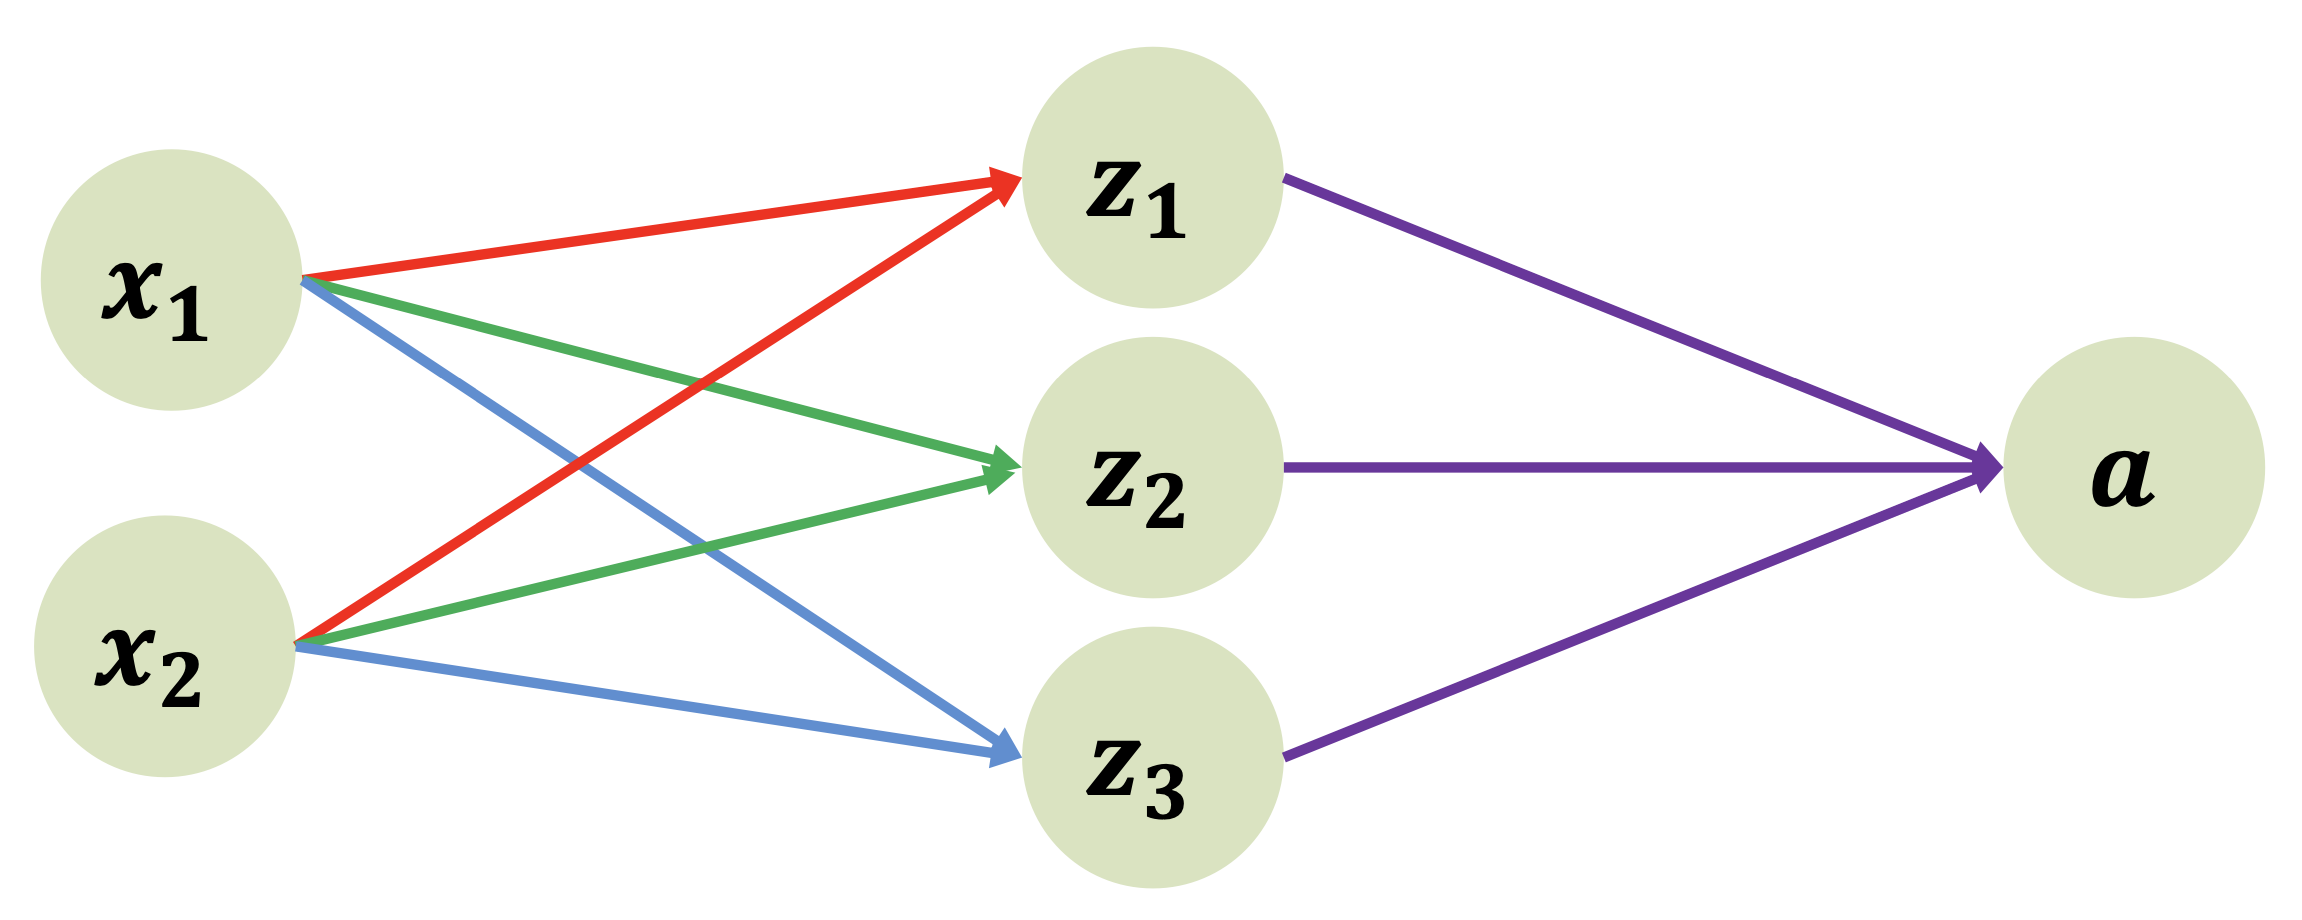
\includegraphics[width=0.7\linewidth]{graph.png}}
                \onslide<6->{\item nodes (vertices) $x_1$ and $x_2$ - features from an input layer of the ANN}
                \onslide<7->{\item nodes (vertices) $z_1$, $z_2$ and $z_3$ - neurons from a hidden layer of the ANN}
                \onslide<8->{\item node (vertex) $a$ - neuron from a output layer of the ANN}
                \onslide<9->{\item Straight lines (edges) correspond to weights between neurons}
            \end{itemize}
        \end{minipage}
    \end{columns}
\end{frame}

%----------------------------------------------------------------------

\begin{frame}
	\frametitle{Human brain}
	It follows the way of human brain processing. ANN modelled how a neuron works in the human brain. So, that’s why it brought into the world of computer science.
	\begin{center}
	    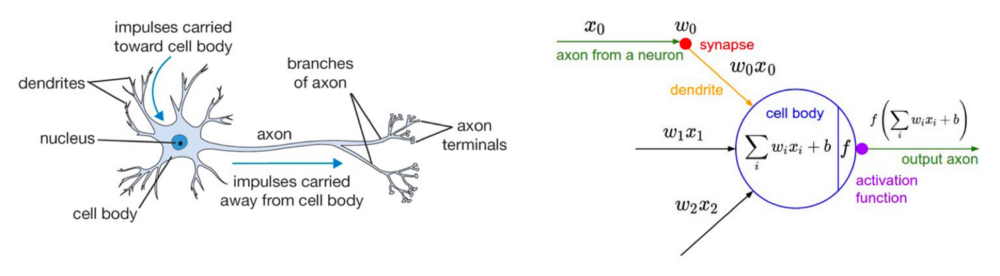
\includegraphics[width=0.9\linewidth]{brain.png}   
	\end{center}
    Neurons on human brain consist of a nucleus, dendrites, cell body, and axon. The number of neurons in humans is approximately 140 billion, consist of 100 billion neurons and 40 billion synapses in neurons. Neurons used to send an impulse to other connected neurons. An impulse is a receptor which getting from sense organs. \href{https://mc.ai/get-to-know-how-artificial-neural-network-formed-in-computer-science/}{\color{blue}\uline{Source}}
\end{frame}

%----------------------------------------------------------------------

\begin{frame}
	\frametitle{How to train?}
	\begin{itemize}
    	\centering
	    \item We know how to train one neuron (e.g. logistic regression): GD or SGD.
	    \item Let’s do the same for the whole network!
	\end{itemize}
\end{frame}

%----------------------------------------------------------------------

\begin{frame}
	\frametitle{GD and SGD: recap}
	\begin{columns}[T]
	    \column{0.5\textwidth}
	    \begin{minipage}[t]{\linewidth}
	        \begin{center}
	            \textbf{Gradient Descent:\\}
                $\theta_{i+1} = \theta_i - \eta \cdot \nabla \red Q \black (\theta_i)$
            \end{center}
            \begin{itemize}
	            \item Pro: Fewer oscillations and noisy steps
	            \item Pro: It produces a more stable gradient descent convergence
	            \item[\textcolor{red}{\textbullet}] Con: A stable error gradient can lead to a local minimum and unlike stochastic gradient descent no noisy steps are there to help get out of the local minimum
	            \item[\textcolor{red}{\textbullet}] Con: It can take too long for processing all the training sample
	        \end{itemize}
        \end{minipage}
		\column{0.5\textwidth}
    	\begin{minipage}[t]{\linewidth}
    	    \begin{center}
                \textbf{Stochastic Gradient Descent:\\}
                $\theta_{i+1} = \theta_i - \eta \cdot \nabla \red Q_j \black (\theta_i)$
            \end{center}
            \begin{itemize}
	            \item Pro: It is computationally fast
	            \item Pro: There are oscillations which can help to get out of local minimums of the loss function
	            \item[\textcolor{red}{\textbullet}] Con: It may take longer to achieve convergence to the minimum of the loss function
	            \item[\textcolor{red}{\textbullet}] Con: Oscillations can lead the gradient descent into other directions
	        \end{itemize}
        \end{minipage}
    \end{columns}
\end{frame}

%----------------------------------------------------------------------

\begin{frame}
    \frametitle{Сomplex function}
	\centering
	How to find the derivative of a complex function?
\end{frame}

%----------------------------------------------------------------------

\begin{frame}
    \frametitle{Chain rule}
	\centering
	\begin{itemize}
    	\centering
	    \item We know how to find the derivative of a simple function.
	    \item Let's remember the rule for differentiating complex functions.
	\end{itemize}
	$\cfrac{\partial f \big(t(x) \big) }{\partial x} = \cfrac{\partial f(t)}{\partial t(x)} \cdot \cfrac{\partial t(x)}{\partial x}$
	\begin{itemize}
	    \centering
    	\item What is the derivative of following function with respect to $x$: $\blue sin(x^2 + 5) \black$?
    	\item What is the derivative of the sigmoid function?
	\end{itemize}
    Can you convert it to $\sigma'(x) = f \big( \sigma(x) \big)$?\\
	\begin{itemize}
	    \centering
	    \item Sigmoid function: $\sigma(x) = \cfrac{1}{1+e^{-x}}$
	\end{itemize}
	\hfill \break
	\onslide<2-> \color{red} Answer: \color{black} $\sigma'(x) = \sigma(x) \cdot \big( 1 - \sigma(x) \big)$
\end{frame}

%----------------------------------------------------------------------

\begin{frame}
	\frametitle{Chain rule for ANN}
	\centering
	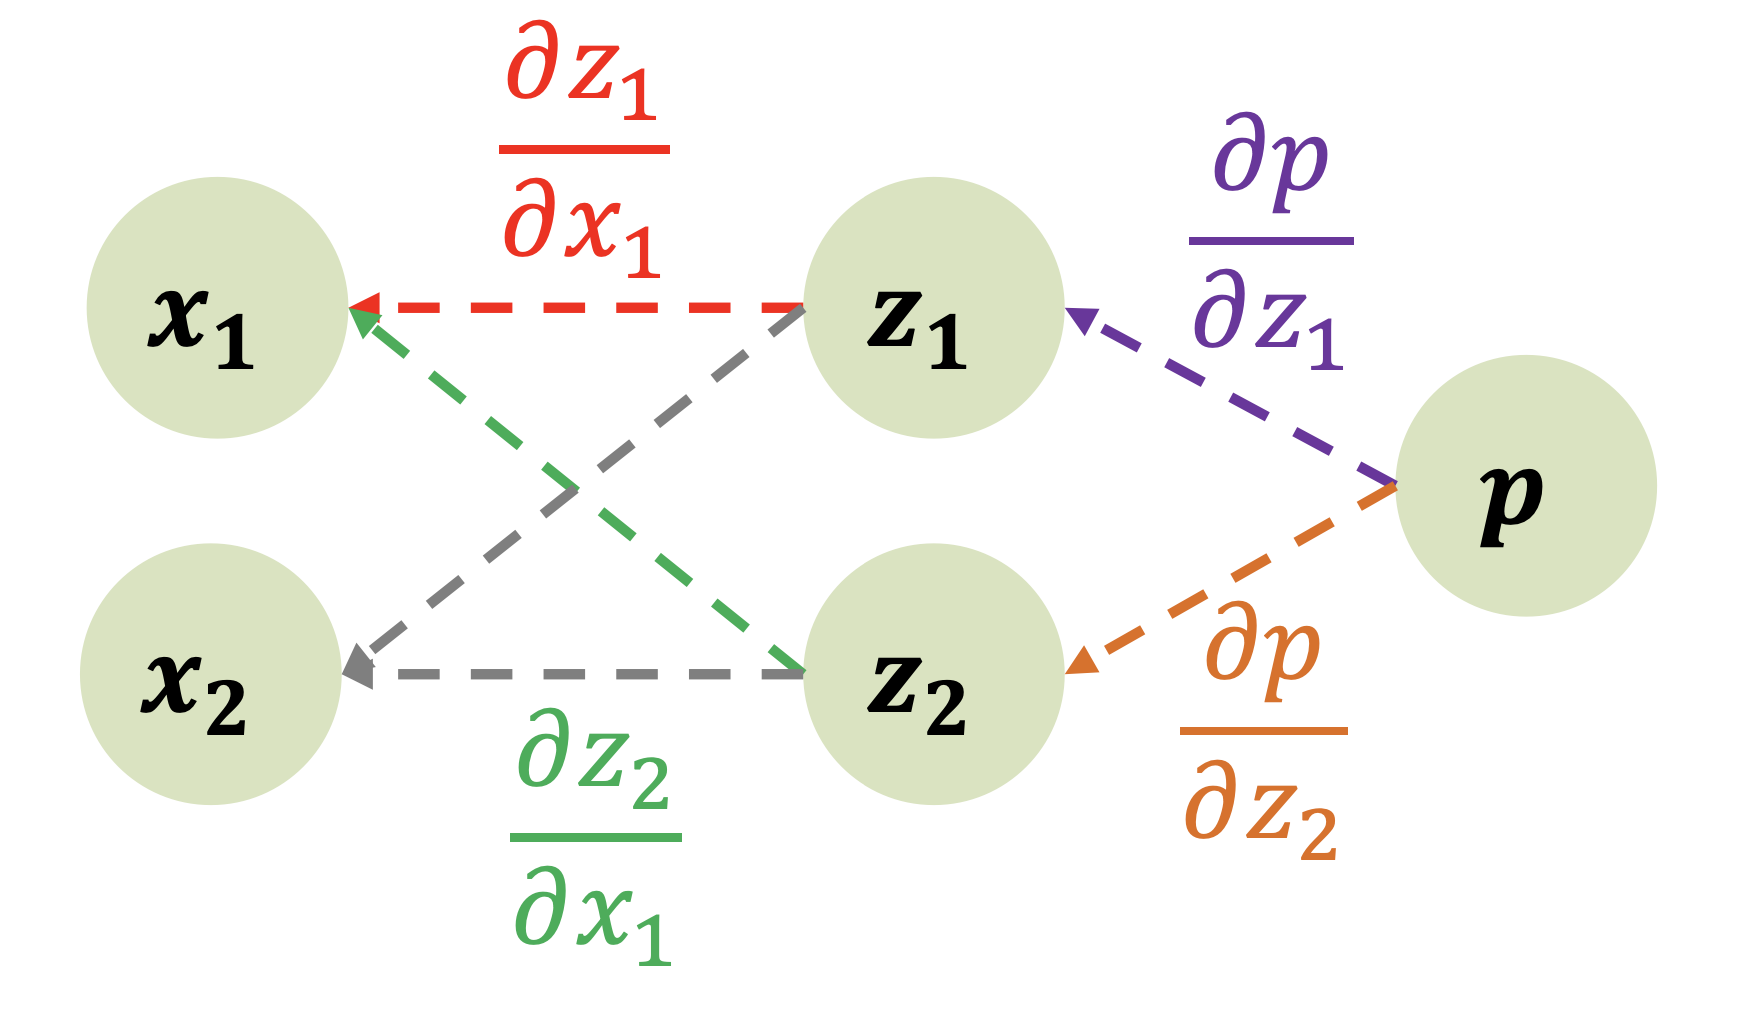
\includegraphics[width=0.5\linewidth]{chain_rule_ann.png}\\
    $\cfrac{\partial p}{\partial x_i} = {\color{violet}\cfrac{\partial p}{\partial z_1}} \cdot {\color{red}\cfrac{\partial z_1}{\partial x_i}} + {\color{orange}\cfrac{\partial p_2}{\partial x_i}} \cdot {\color{green}\cfrac{\partial z_2}{\partial x_i}}$
    \vspace{0.3em},\\
    where $x_{i}$ is $x_{1}$ or $x_{2}$
\end{frame}

%----------------------------------------------------------------------

\begin{frame}
	\frametitle{Back propagation}
	\centering
    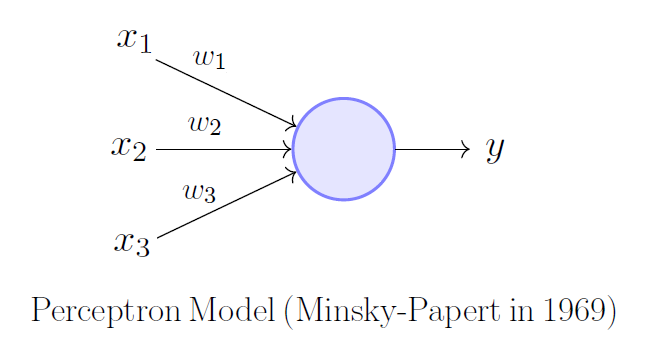
\includegraphics[width=0.35\linewidth]{perceptron_model.png}\\
    \href{https://towardsdatascience.com/what-is-a-perceptron-210a50190c3b}{\color{blue}\uline{Source}}\\
    $Q \big(y_{model}, y_{target} \big) = Q \big(y(x, w, b), y_{target} \big)$\\
    $out = y = \sigma \big(sum \big)= \sigma \big(\sum \limits_{i=1}^{3}(x_i \cdot w_i) + b \big)$
    $\cfrac{\partial Q}{\partial w_i} = \cfrac{\partial Q}{\partial y} \cdot \cfrac{\partial y}{\partial \sigma} \cdot \cfrac{\partial \sigma}{\partial sum} \cdot \cfrac{\partial sum}{\partial w_i} = \cfrac{\partial Q}{\partial y} \cdot \red 1 \black \cdot \cfrac{\partial \sigma}{\partial sum} \cdot \cfrac{\partial sum}{\partial w_i}$\\
    $\cfrac{\partial \sigma}{\partial sum} = \sigma (sum) \cdot \big(1 - \sigma (sum) \big)$
\end{frame}

%----------------------------------------------------------------------

\begin{frame}
	\frametitle{Back propagation: an example}
	\centering
	\begin{columns}[T]
	    \column{0.5\textwidth}
	    \begin{minipage}[t]{\linewidth}
	        \centering
	        $Q \big(y(x, w, b), y_{target} \big)$\\
	        $Q = \big(y_{target} - y(x_1, w_1, b) \big)^2$\\
	        $out = y = (x \cdot w) + b$\\
	        $\cfrac{\partial Q}{\partial w_i} = \cfrac{\partial Q}{\partial y} \cdot \cfrac{\partial y}{\partial w_i}$\\
            Input: x = 1, w = 0.1 and b = 1\\
            $y_{target} = 2$ and learning rate: $\eta = 0.1$\\
            \onslide<2->{\blue How to find $w_{new}$ and $b_{new}$? \black}
        \end{minipage}
		\column{0.5\textwidth}
    	\begin{minipage}[t]{\linewidth}
    	    \centering
            \onslide<2->{$\cfrac{\partial Q}{\partial y} = -2 \cdot (y_{target} - y)$\\
            $\cfrac{\partial Q}{\partial w} = \cfrac{\partial Q}{\partial y} \cdot \cfrac{\partial y}{\partial w} = -2 \cdot x \cdot (y_{target} - y)$\\
            $\cfrac{\partial Q}{\partial b} = \cfrac{\partial Q}{\partial y} \cdot \cfrac{\partial y}{\partial b} = -2 \cdot (y_{target} - y)$\\
            $ \blue [w_{new}, b_{new}] \black \Rightarrow \theta_{i+1} = \theta_i - \eta \cdot \cfrac{\partial Q(\theta_i)}{\partial \theta_i}$\\}
        \end{minipage}
    \end{columns}
    \hfill \break
    \hfill \break
    \onslide<3->{\begin{tabular}{ |p{1cm}|p{1cm}|p{1cm}|p{1cm}|p{1cm}|p{1cm}|p{1cm}| }
                     \hline
                     y & Q & $\cfrac{\partial Q}{\partial y}$ & $\cfrac{\partial Q}{\partial w}$ &  $\cfrac{\partial Q}{\partial b}$ & $w_{new}$ & $b_{new}$\\
                     \hline
                     1.1 & 0.81 & -1.8 & -1.8 & -1.8 & 0.28 & 1.18\\
                     \hline
                 \end{tabular}}
\end{frame}

%----------------------------------------------------------------------

\begin{frame}
	\frametitle{Momentum and Root Mean Square Propagation (RMSProp)}
	\begin{columns}[T]
	    \column{0.5\textwidth}
	    \begin{minipage}[t]{\linewidth}
	        \centering
	        \begin{center}
	            \textbf{SGD with momentum:}
            \end{center}
	        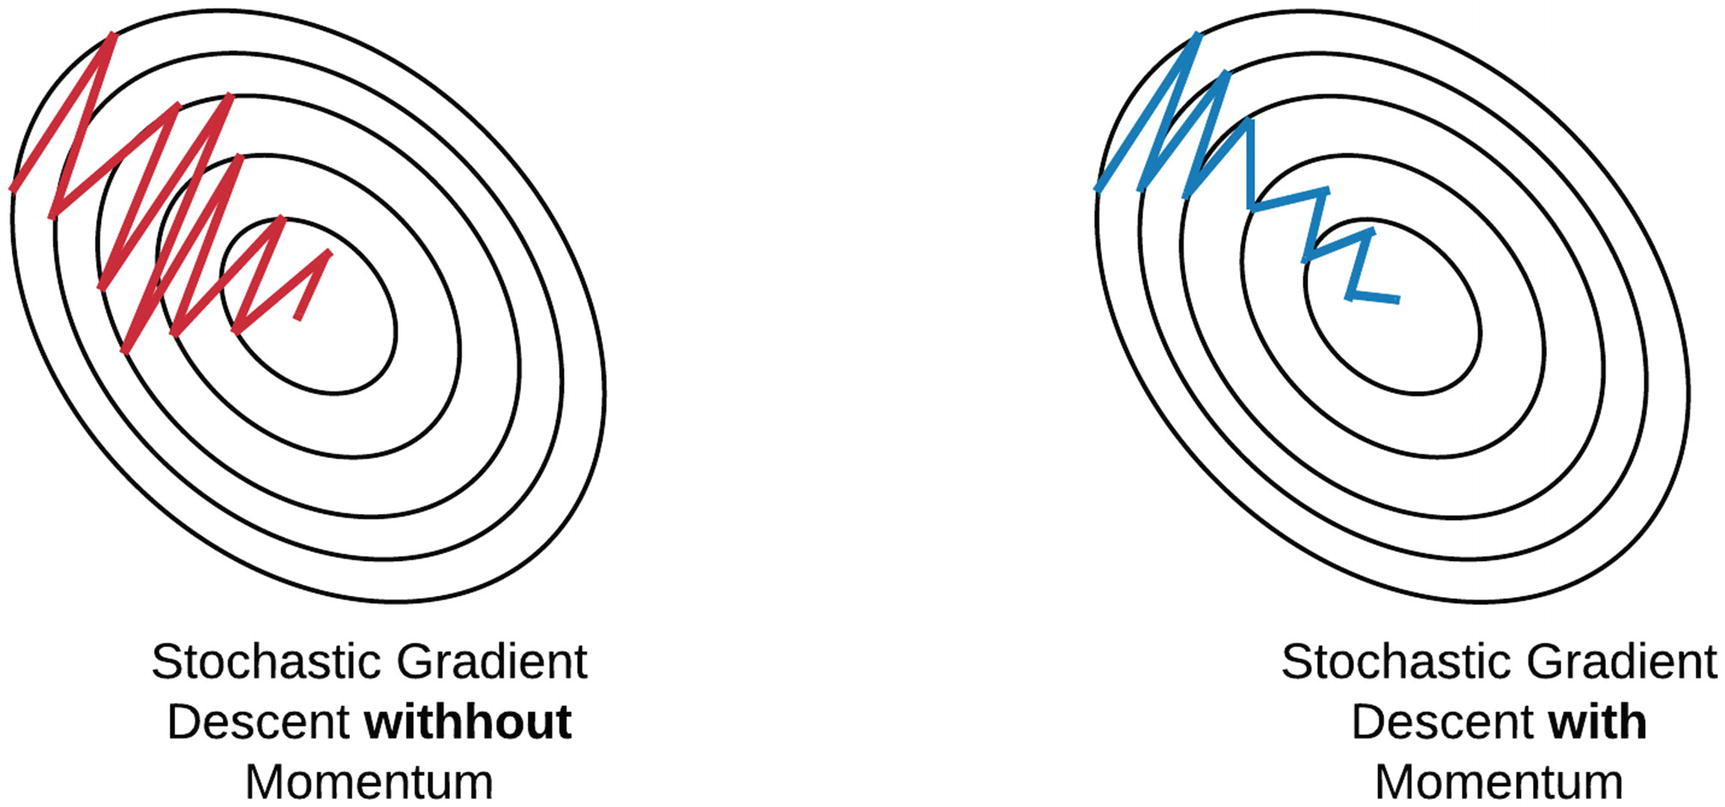
\includegraphics[width=0.6\linewidth]{momentum.png}\\
		    \href{https://eloquentarduino.github.io/2020/04/stochastic-gradient-descent-on-your-microcontroller/}{\color{blue}\uline{Source}}\\
		    $\theta_{i+1} = \theta_i - \Delta \theta_{i+1}$\\
		    $\Delta \theta_{i+1} = \alpha \cdot \Delta \theta_i + \eta \cdot \nabla Q_j(\theta_i)$\\
		    \begin{itemize}
		        \item $\alpha$ is an exponential decay factor between 0 and 1 that determines the relative contribution of the current gradient and earlier gradients to the weight change
		    \end{itemize}
        \end{minipage}
		\column{0.5\textwidth}
    	\begin{minipage}[t]{\linewidth}
    	    \centering
    	    \begin{center}
	            \textbf{RMSProp:}
            \end{center}
            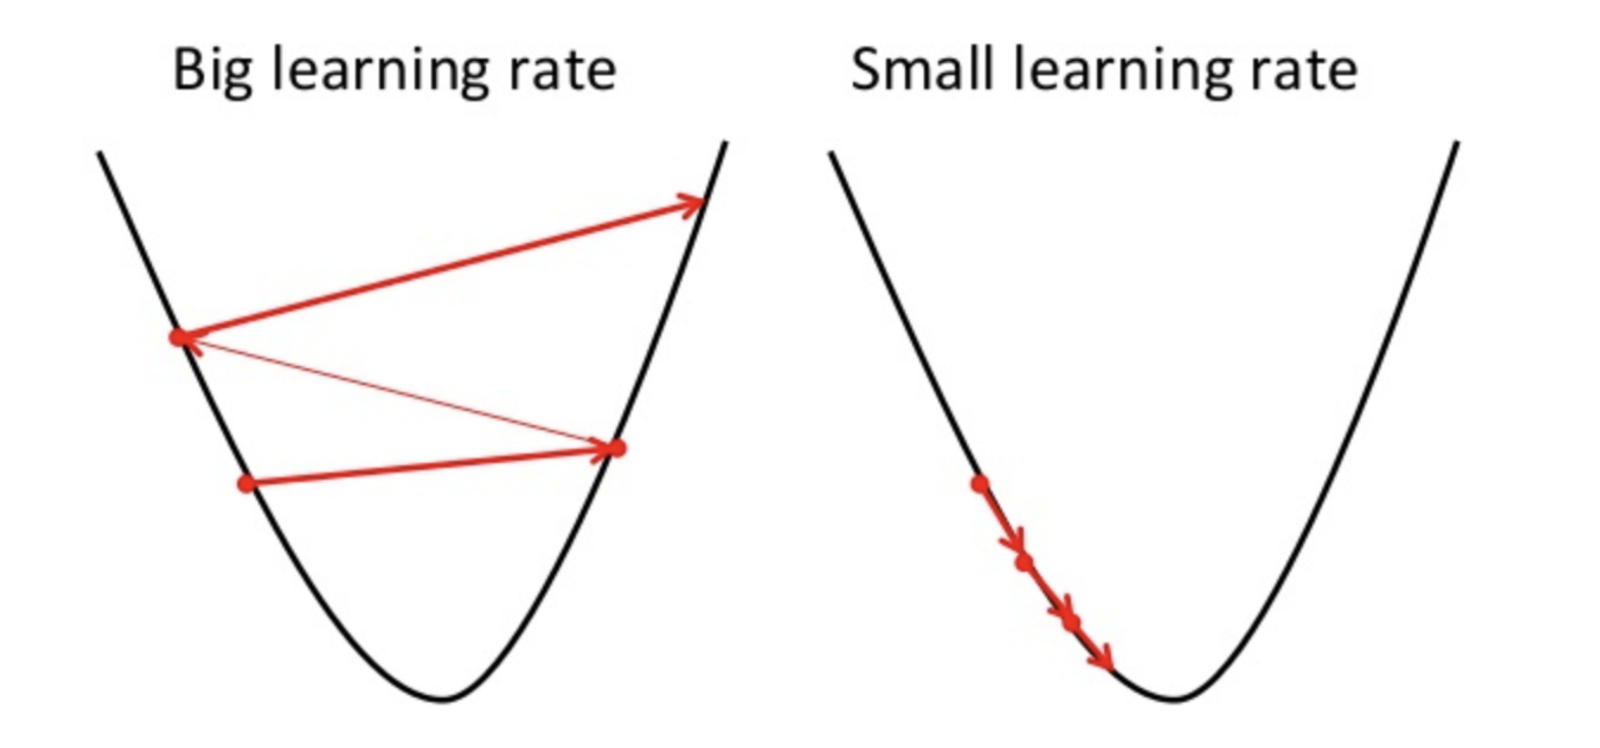
\includegraphics[width=0.7\linewidth]{rmsprop.png}\\
		    \href{https://deepai.org/machine-learning-glossary-and-terms/rmsprop}{\color{blue}\uline{Source}}\\
    	    $\theta_{i+1} = \theta_i - \cfrac{\eta}{\sqrt{v_{i+1} + \blue \bm \epsilon \black} + \red \bm \epsilon \black} \cdot \nabla Q_j(\theta_i)$\\
		    $v_{i+1} = \rho \cdot v_i + (1 - \rho) \cdot \big(\nabla Q_j(\theta_i) \big)^2$\\
		    \begin{itemize}
		        \item $\rho$ is moving average parameter (the forgetting factor)
		    \end{itemize}
        \end{minipage}
    \end{columns}
\end{frame}

%----------------------------------------------------------------------

\begin{frame}
	\frametitle{Nesterov momentum and Adaptive Moment Estimation (Adam)}
	\begin{columns}[T]
	    \column{0.5\textwidth}
	    \begin{minipage}[t]{\linewidth}
	        \centering
	        \begin{center}
	            \textbf{SGD with nesterov momentum:}
            \end{center}
	        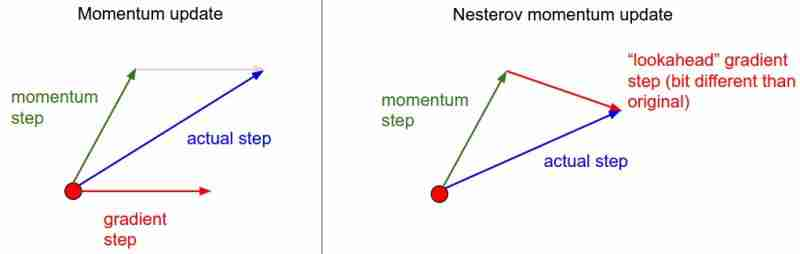
\includegraphics[width=1.0\linewidth]{nesterov.png}\\
		    \href{https://mc.ai/ml-advancedmomentum-in-machine-learning-what-is-nesterov-momentum/}{\color{blue}\uline{Source}}\\
		    $\theta_{i+1} = \theta_i - \Delta \theta_{i+1}$\\
		    $\Delta \theta_{i+1} = \alpha \cdot \Delta \theta_i + \eta \cdot \nabla Q_j(\theta_i - \alpha \cdot \Delta \theta_i)$\\
        \end{minipage}
		\column{0.5\textwidth}
    	\begin{minipage}[t]{\linewidth}
    	    \centering
    	    \begin{center}
	            \textbf{Adam and Nadam:}
            \end{center}
            \hfill \break
            \begin{itemize}
                \item Adam optimizer is essentially RMSProp with momentum
                \item Nadam optimizer is Adam with Nesterov momentum
            \end{itemize}
        \end{minipage}
    \end{columns}
\end{frame}

%----------------------------------------------------------------------

\begin{frame}
	\frametitle{Break time = this is big brain time}
	\centering
	
\includegraphics[width=0.4\linewidth]{big_brain_time.jpg}\\
	\begin{itemize}
    	\centering
	    \item Is it necessary to use a bias neuron and why?
	    \item What values can the weights of neurons take?
	\end{itemize}
\end{frame}

%----------------------------------------------------------------------

\begin{frame}
	\centering
	\large \textbf{Deep Learning}\\
	!!!!!!!!!!!!!!!!!!!!!!!!!!!!!!!!!!!!ADD LINKS!!!!!!!!!!!!!!!!!!!!!!!!!!!!!!!!!!!!
\end{frame}

%----------------------------------------------------------------------

\begin{frame}[t]
\frametitle{Motivation}
\begin{columns}[T]
	\column{0.5\textwidth}
	\begin{minipage}[t]{\linewidth}
		\centering 
		Let's take a look at the human brain
		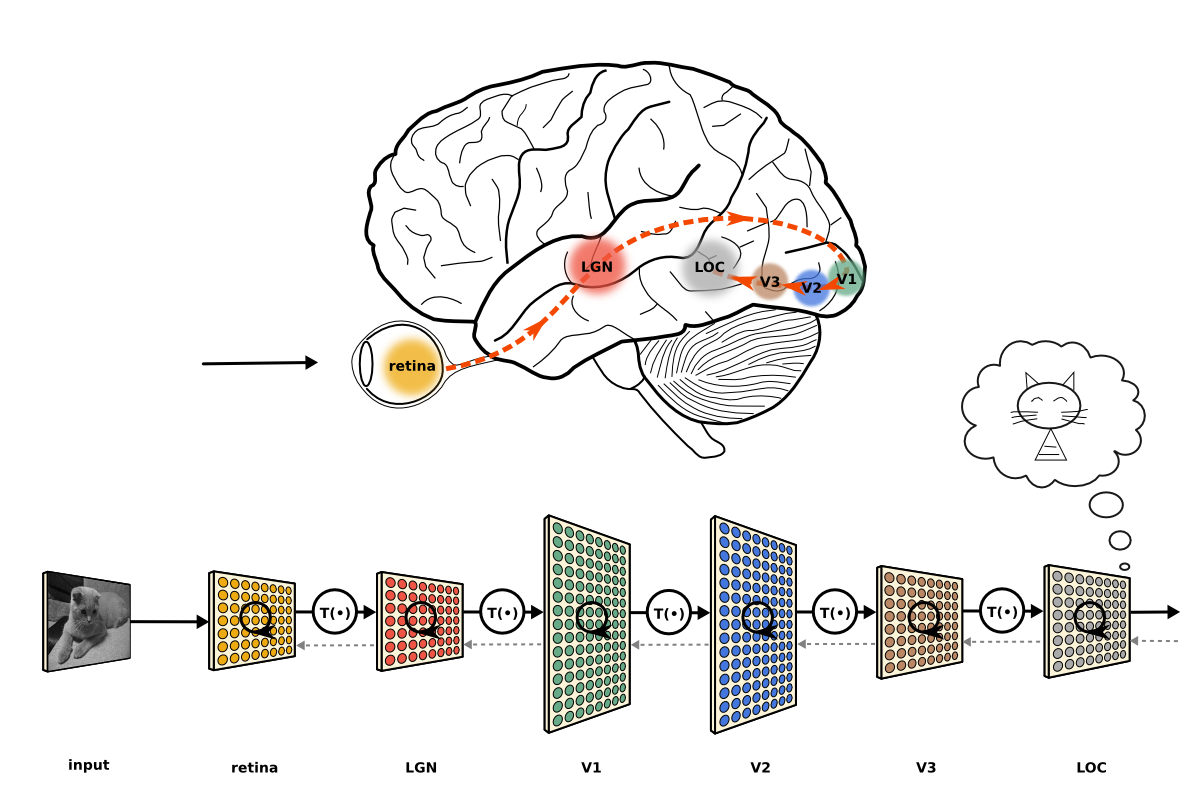
\includegraphics[width=0.9\linewidth]{visual_stream}
		\vspace{-0.5em}
		\begin{itemize}
			\item Visual signals travel through multiple areas of a different organization
			\item This makes our visual system incredibly robust 
		\end{itemize}
	\end{minipage}%	
	\column{0.5\textwidth}
	\begin{minipage}[t]{\linewidth}
		\centering
		The same approach is valid for ANN:\\
		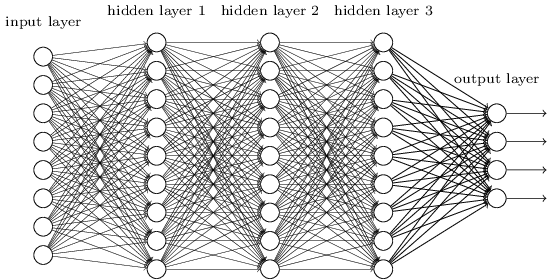
\includegraphics[width=1\linewidth]{DNN}\\
		\href{http://neuralnetworksanddeeplearning.com/chap5.html}{\color{blue}\uline{Source}}\\
		\vspace{0.5em}
		Deep Learning  $\Leftrightarrow$ complex models?\\
		\onslide<2->{\red Not exactly!}
	\end{minipage}
\end{columns}
\end{frame}

%----------------------------------------------------------------------

\begin{frame}[t]
	\frametitle{The meaning of "Deep"}
	\begin{columns}[T]
		\column{0.5\textwidth}
		\begin{minipage}[T]{\linewidth}
			\begin{itemize}
				\item Dummy explanation refers to a number of layers ($\text{N}_{\ell} \geq 3 \Rightarrow$ DNN)
				\item More profound viewpoint:\\
				\textit{Deep learning is a deep understanding of data structure}
				\item Here is an example:
			\end{itemize}
		\end{minipage}%	
		\column{0.5\textwidth}
		\begin{minipage}[T]{\linewidth}
			\centering
			\begin{itemize}
				\onslide<3->\item Input data contain high and low-level features
				\onslide<4->\item We don't know the exact set of features and need to invent them
				\onslide<5->\item ANN has lots of inputs 
				\onslide<6->\item \color{blue} See the next lecture on more complex ANN \color{black}
			\end{itemize}
		\end{minipage}
	\end{columns}
\onslide<2-> \centering 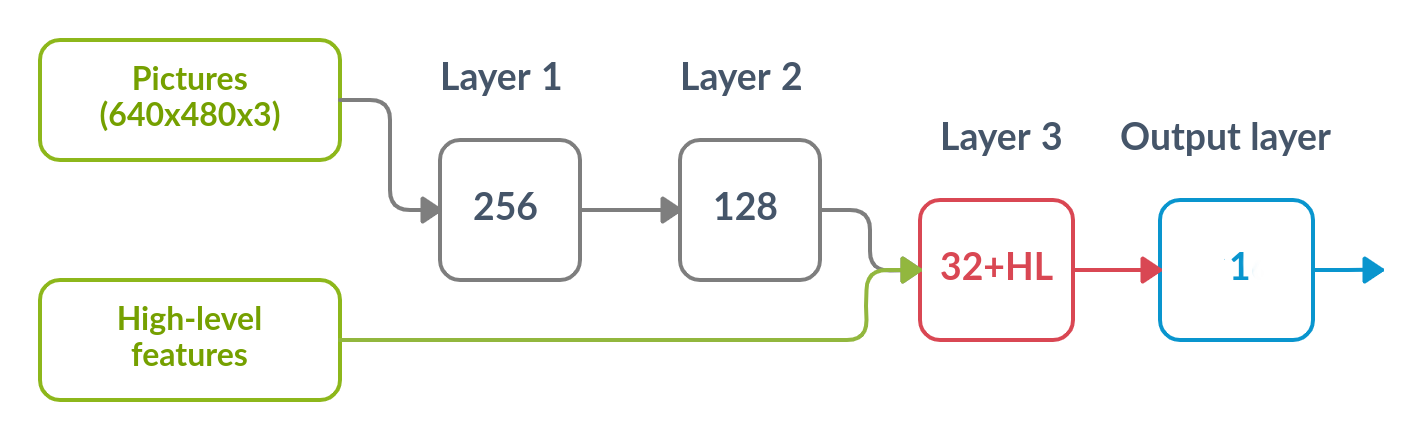
\includegraphics[width=0.7\linewidth]{DNN_example}
\end{frame}

%----------------------------------------------------------------------

\begin{frame}[t]
	\frametitle{The Achilles heel of the DL models}
	\begin{columns}
		\column{0.5\textwidth}
		\begin{minipage}[t]{\linewidth}
			\begin{itemize}
				\item Train a DNN with the SGD method
				\onslide<2->\item Layer $f_i(\bm{z_{i-1}})$ takes the output $\bm{z_{i-1}}$ from the previous layer and returns $\bm{z_i}$
				\onslide<3->\item Making backprop we calculate: \\ $\cfrac{\partial Q}{\partial \omega_j} = \cfrac{\partial Q}{\partial f_i}\cfrac{\partial f_i}{\partial f_{i-1}}\cdots \cfrac{\partial f_{1}}{\partial \omega_j}$
				\onslide<4->\item Here $\cfrac{\partial f_i}{\partial f_{i-1}} = \sigma(z_{i-1})\big(1-\sigma(z_{i-1})\big)$
				\onslide<5->\item $\bigg|\cfrac{\partial f_i}{\partial f_{i-1}}\bigg| \leq \cfrac{1}{4} \Rightarrow \Delta \omega_i \rightarrow 0$
			\end{itemize}
		\end{minipage}%	
		\column{0.5\textwidth}
		\begin{minipage}[t]{\linewidth}
		\flushleft
		\onslide<1->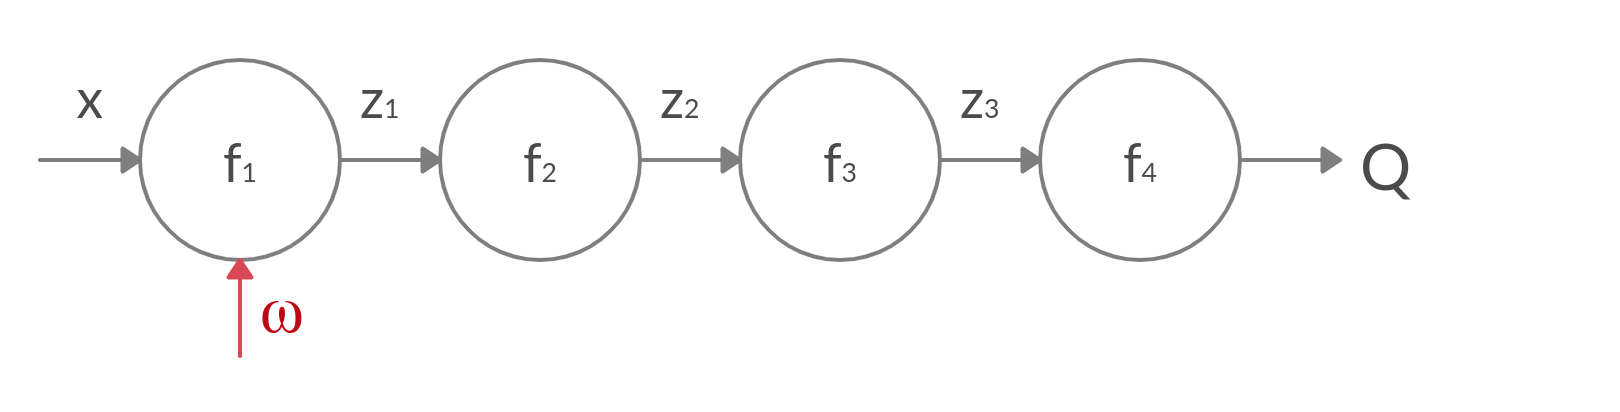
\includegraphics[width=1\linewidth]{vanishing_grad_NN}\\
		\vspace{-0.5em}
		\onslide<4->\hspace{-1em}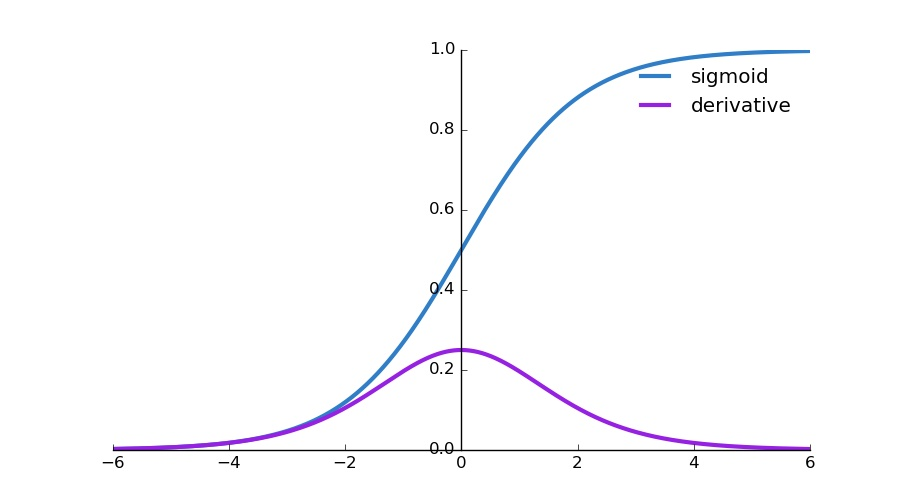
\includegraphics[width=0.9\linewidth]{sigmoid_der.jpg}
		\end{minipage}
	\end{columns}
	\vspace{1em}
 	\onslide<6->\centering \red Problem: \black Gradient step vanishes for the initial layers $\Rightarrow$ undertraining! 
\end{frame} 

%----------------------------------------------------------------------

\begin{frame}[t]
	\frametitle{The Achilles heel of the DL models}
	\begin{columns}[T]
		\column{0.5\textwidth}
		\begin{minipage}[T]{\linewidth}
			An artificial example:
			\begin{itemize}
				\onslide<2->\item Initialize all $\omega_j$ = 100 (\red bad\black)
				\onslide<3->\item Choose all biases that all $z_i = 0$
				\onslide<4->\item Then each $\cfrac{\partial f_i}{\partial f_{i-1}} = \cfrac{1}{4}$
				\onslide<5->\item $\Delta \omega_j = \bigg(100\cdot\cfrac{1}{4}\bigg)^{N-j+1},$\\
				\vspace{0.3em} where $N$ is a total number of layers
				\onslide<6->\item[\red \textbullet] Exploding and vanishing gradients evidence the problem of model instability
			\end{itemize}
		\end{minipage}%	
		\column{0.5\textwidth}
		\begin{minipage}[T]{\linewidth}
			\centering
			\onslide<1->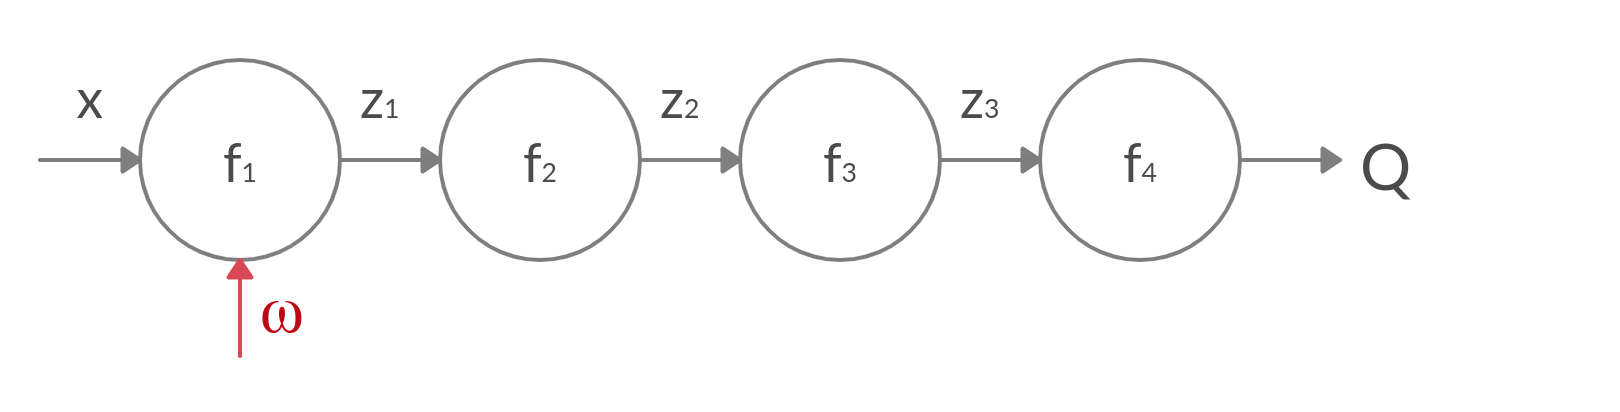
\includegraphics[width=1\linewidth]{vanishing_grad_NN}\\
			\vspace{-0.5em}
			\onslide<5->\hspace{-1em}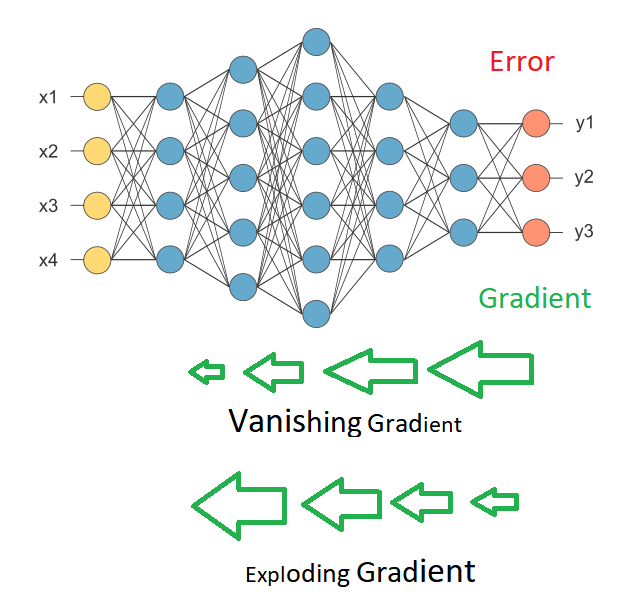
\includegraphics[width=0.7\linewidth]{unstable_grad_NN}
		\end{minipage}
	\end{columns}
	\vspace{1em}
\end{frame} 

%----------------------------------------------------------------------

\begin{frame}[t]
	\frametitle{Reaching stability}
	\vspace{0.5em}
	\begin{columns}[T]
		\column{0.5\textwidth}
		\begin{minipage}[T]{\linewidth}
			\begin{itemize}
				\item Different activation functions (ReLU)
				\onslide<2->\item Regularization of network architecture
				\onslide<3->{\item Normalization:
				\begin{itemize}
					\item Input variables (\red data preprocessing\black)
					\item Batch normalization
				\end{itemize}}
			\onslide<4->\item Different training methods
			\end{itemize}%
		\vspace{1.5em}
		\onslide<5->{We'll partially cover them at this lecture}
			
		\end{minipage}%
		\column{0.5\textwidth}
		\begin{minipage}[T]{\linewidth}
			\centering
			\onslide<1->\vspace{-1em}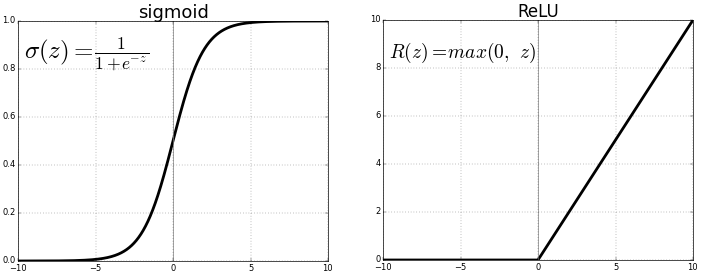
\includegraphics[width=0.8\linewidth]{sig_relu}\\
			\onslide<2->\vspace{0.5em} 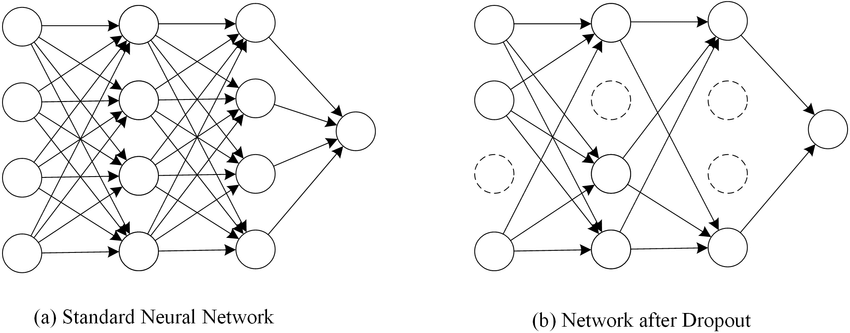
\includegraphics[width=0.7\linewidth]{dropout}
			\onslide<3-> 	\vspace{0.5em}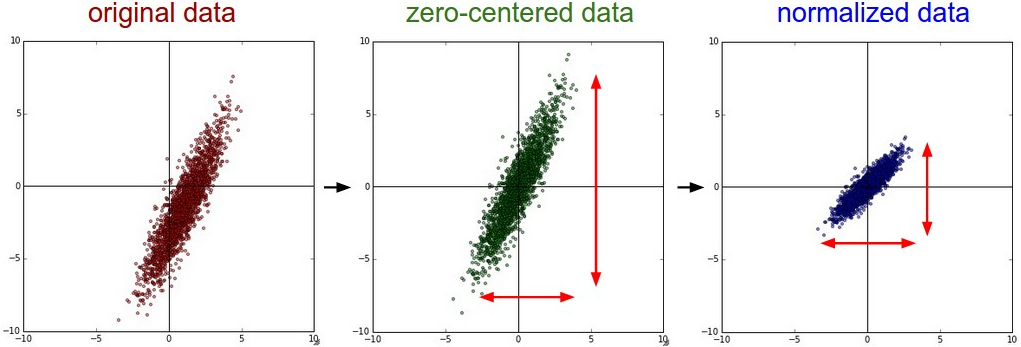
\includegraphics[width=0.8\linewidth]{normalization}\\
		\end{minipage}
	\end{columns}
\end{frame}

%----------------------------------------------------------------------

\begin{frame}[t]
	\frametitle{Activation functions: Sigmoid and Rectified Linear Unit (ReLU)}
	\vspace{0.5em}
	\begin{columns}[T]
		\column{0.5\textwidth}
		\begin{minipage}[T]{\linewidth}
			\centering
				\vspace{-1em}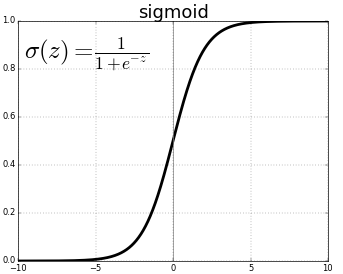
\includegraphics[width=0.5\linewidth]{sigmoid.png}\\
			\begin{itemize}
				\item Differentiable
				\item Shrinks parameter domain into $[0,1]$
				\item $|\sigma'(x)| \leq \cfrac{1}{4}$
			\end{itemize}%
		\end{minipage}%
		\column{0.5\textwidth}
		\begin{minipage}[T]{\linewidth}
			\centering
			\vspace{-1em}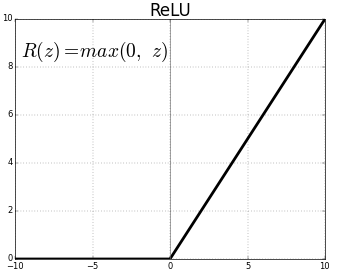
\includegraphics[width=0.5\linewidth]{relu.png}\\
			\begin{itemize}
				\item Non-differentiable at 0, but we still can define $R'(0) \coloneqq 0~\text{or}~1$
				\item Shrinks parameter domain into $\mathbb{R^+}$\\
				\item $R'(x)\in \{0,1\}$
				\item There are different variations of ReLU: Leaky ReLU, Parametric ReLU (PReLU), Exponential ReLU (ELU), ...
			\end{itemize}
		\end{minipage}
	\end{columns}
\end{frame}

%----------------------------------------------------------------------

\begin{frame}[t]
	\frametitle{Activation functions: Tanh and Swish}
	\vspace{0.5em}
	\begin{columns}[T]
		\column{0.5\textwidth}
		\begin{minipage}[T]{\linewidth}
			\centering
				\vspace{-1em}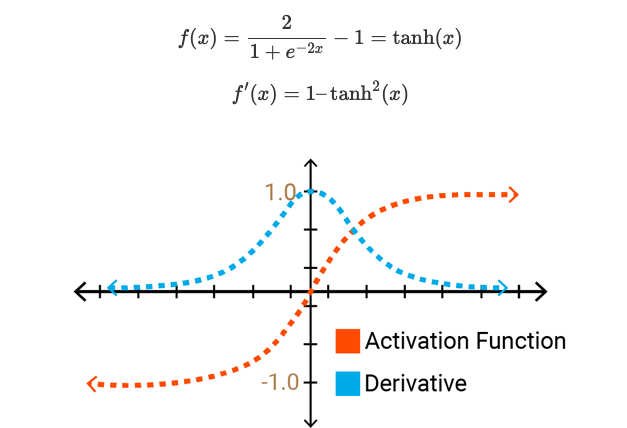
\includegraphics[width=0.6\linewidth]{tanh_and_tanh_der.png}\\
			\begin{itemize}
		    	\item Hyperbolic Tangent Function: $\tanh(x) = \cfrac{e^{x} - e^{-x}}{e^{x} + e^{-x}}$
				\item Differentiable
				\item Shrinks parameter domain into $[-1,1]$
				\item $|\tanh'(x)| \leq 1$
			\end{itemize}%
		\end{minipage}%
		\column{0.5\textwidth}
		\begin{minipage}[T]{\linewidth}
			\centering
			\vspace{-1em}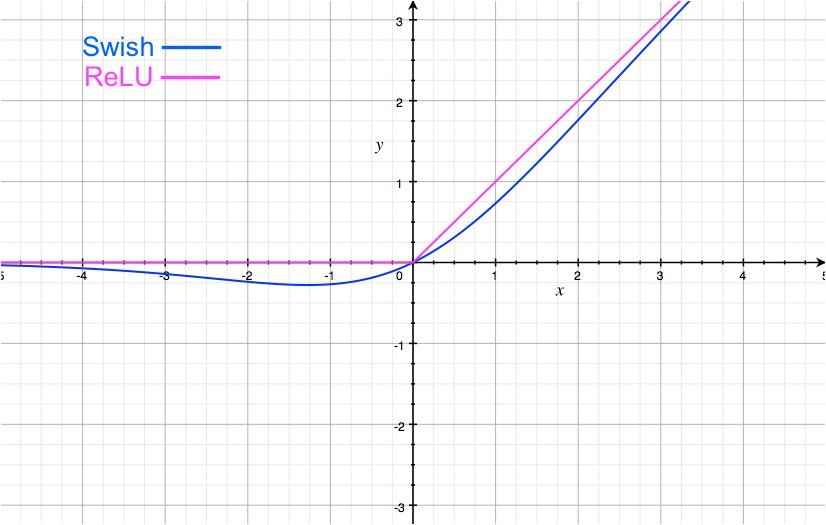
\includegraphics[width=0.5\linewidth]{swish.png}\\
			\begin{itemize}
		    	\item swish(x) $= \cfrac{x}{1+e^{-\beta \cdot x}} = x \cdot \sigma(\beta \cdot x)$
				\item Differentiable
				\item $\beta \rightarrow 1 \Rightarrow$ Sigmoid Linear Unit (SiLU)
				\item $\beta \rightarrow 0 \Rightarrow$ swish(x) $= \cfrac{x}{2}$
				\item $\beta \rightarrow \infty \Rightarrow$ swish(x) $\sim ReLU$
			\end{itemize}
		\end{minipage}
	\end{columns}
\end{frame}

%----------------------------------------------------------------------

\begin{frame}[t]
	\frametitle{Regularization: two common methods}
	\vspace{-0.5em}
	\begin{columns}[t]
		\column{0.5\textwidth}
		\begin{minipage}[t]{\linewidth}
			\centering L2 regularization (Tikhonov)\\
			\vspace{1em}
			$Q(a)=\frac{1}{N}\sum\limits_{j=1}^{N}\big(\langle\bm{x},\bm{\beta}\rangle - y_j\big)^2 \color{calmRed}+ \lambda \sum\limits_{i=1}^{K}(\bm\beta_i)^2 $
		\end{minipage}%
		\column{0.5\textwidth}
		\begin{minipage}[t]{\linewidth}
			\centering L1 regularization (LASSO)\\
			\tiny{\color{gray}least absolute shrinkage and selection operator}
			\normalsize
			$Q(a) = \frac{1}{N}\sum\limits_{j=1}^{N}\big(\langle\bm{x},\bm{\beta}\rangle - y_j\big)^2 \color{calmRed} + \lambda \sum\limits_{i=1}^{K}|\bm\beta_i| $
		\end{minipage}%
	\end{columns}
	\centering 
	\vspace{0.5em}
	The red term brings up a penalty when the model includes lots of terms\\or the weights are too high\\
	\begin{columns}[t]
		\column{0.5\textwidth}
		\centering
		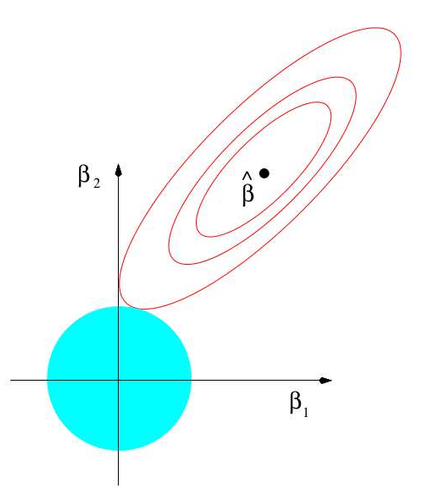
\includegraphics[width=0.4\linewidth]{ridge}
		%	\begin{itemize}
		%		\item Punish the terms with high values
		%		\item Fails to perform variable selection
		%	\end{itemize}
		\column{0.5\textwidth}
		\centering
		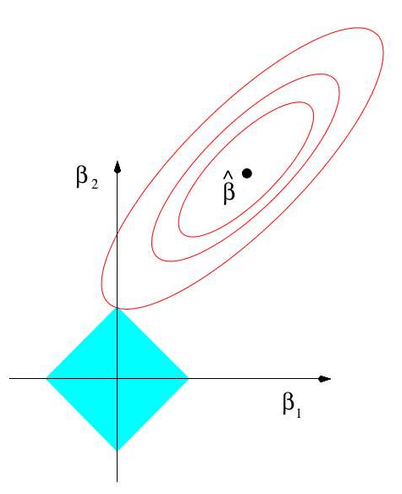
\includegraphics[width=0.4\linewidth]{lasso}
		%	\begin{itemize}
		%		\item Punish terms more uniformly since linearly depends on the weight value
		%		\item Works well in variable selection
		%		
		%	\end{itemize}
	\end{columns}
\end{frame}

%----------------------------------------------------------------------

\begin{frame}[t]
	\frametitle{Regularization: Dropout}
	\vspace{0.5em}
	\begin{columns}
		\column{0.5\textwidth}
		\begin{minipage}[T]{\linewidth}
			\begin{itemize}
				\setbeamertemplate{items}{\color{DESYBlue}{\rotatebox[origin=c]{-90}{\MVRightarrow}}}
				\item Initialize a fully connected network
				\item With probability $p$ switch off neurons
				\item Train this architecture
				\item Repeat for several configurations and take average results for weights $\bm \omega$
				\item Apply weights to a fully connected network and modify activation function: $a'(\bm x, \bm \omega) = (1-p) a(\bm x, \bm \omega)$
			\end{itemize}%
		\end{minipage}%
		\column{0.5\textwidth}
		\begin{minipage}[T]{\linewidth}
			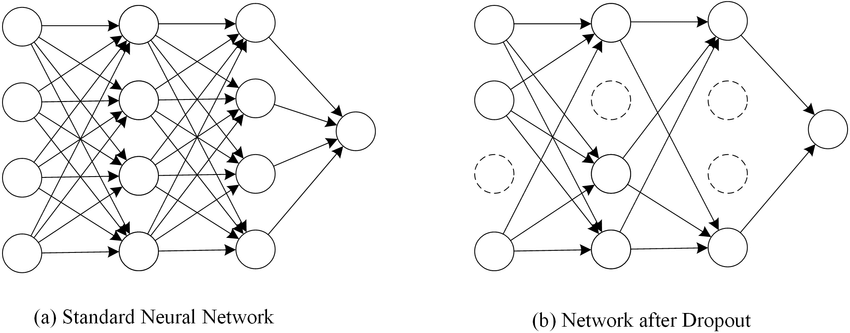
\includegraphics[width=1\linewidth]{dropout}\\
			\flushleft
			\green Dropout \black prevents complex co-adaptations of neurons and provides reasonable improvement of ANN results.\\
			\href{https://arxiv.org/pdf/1207.0580.pdf}{\color{blue}\uline{Original article}}
		\end{minipage}
	\end{columns}
\end{frame}

%----------------------------------------------------------------------

\begin{frame}
	\centering
	\large ANN architectures' examples\\
	\href{https://www.asimovinstitute.org/neural-network-zoo/}{\color{blue}\uline{Source}}
\end{frame}

%----------------------------------------------------------------------

\begin{frame}[t]
	\frametitle{Network architectures}
	\centering
	\vspace{-0.5em}
	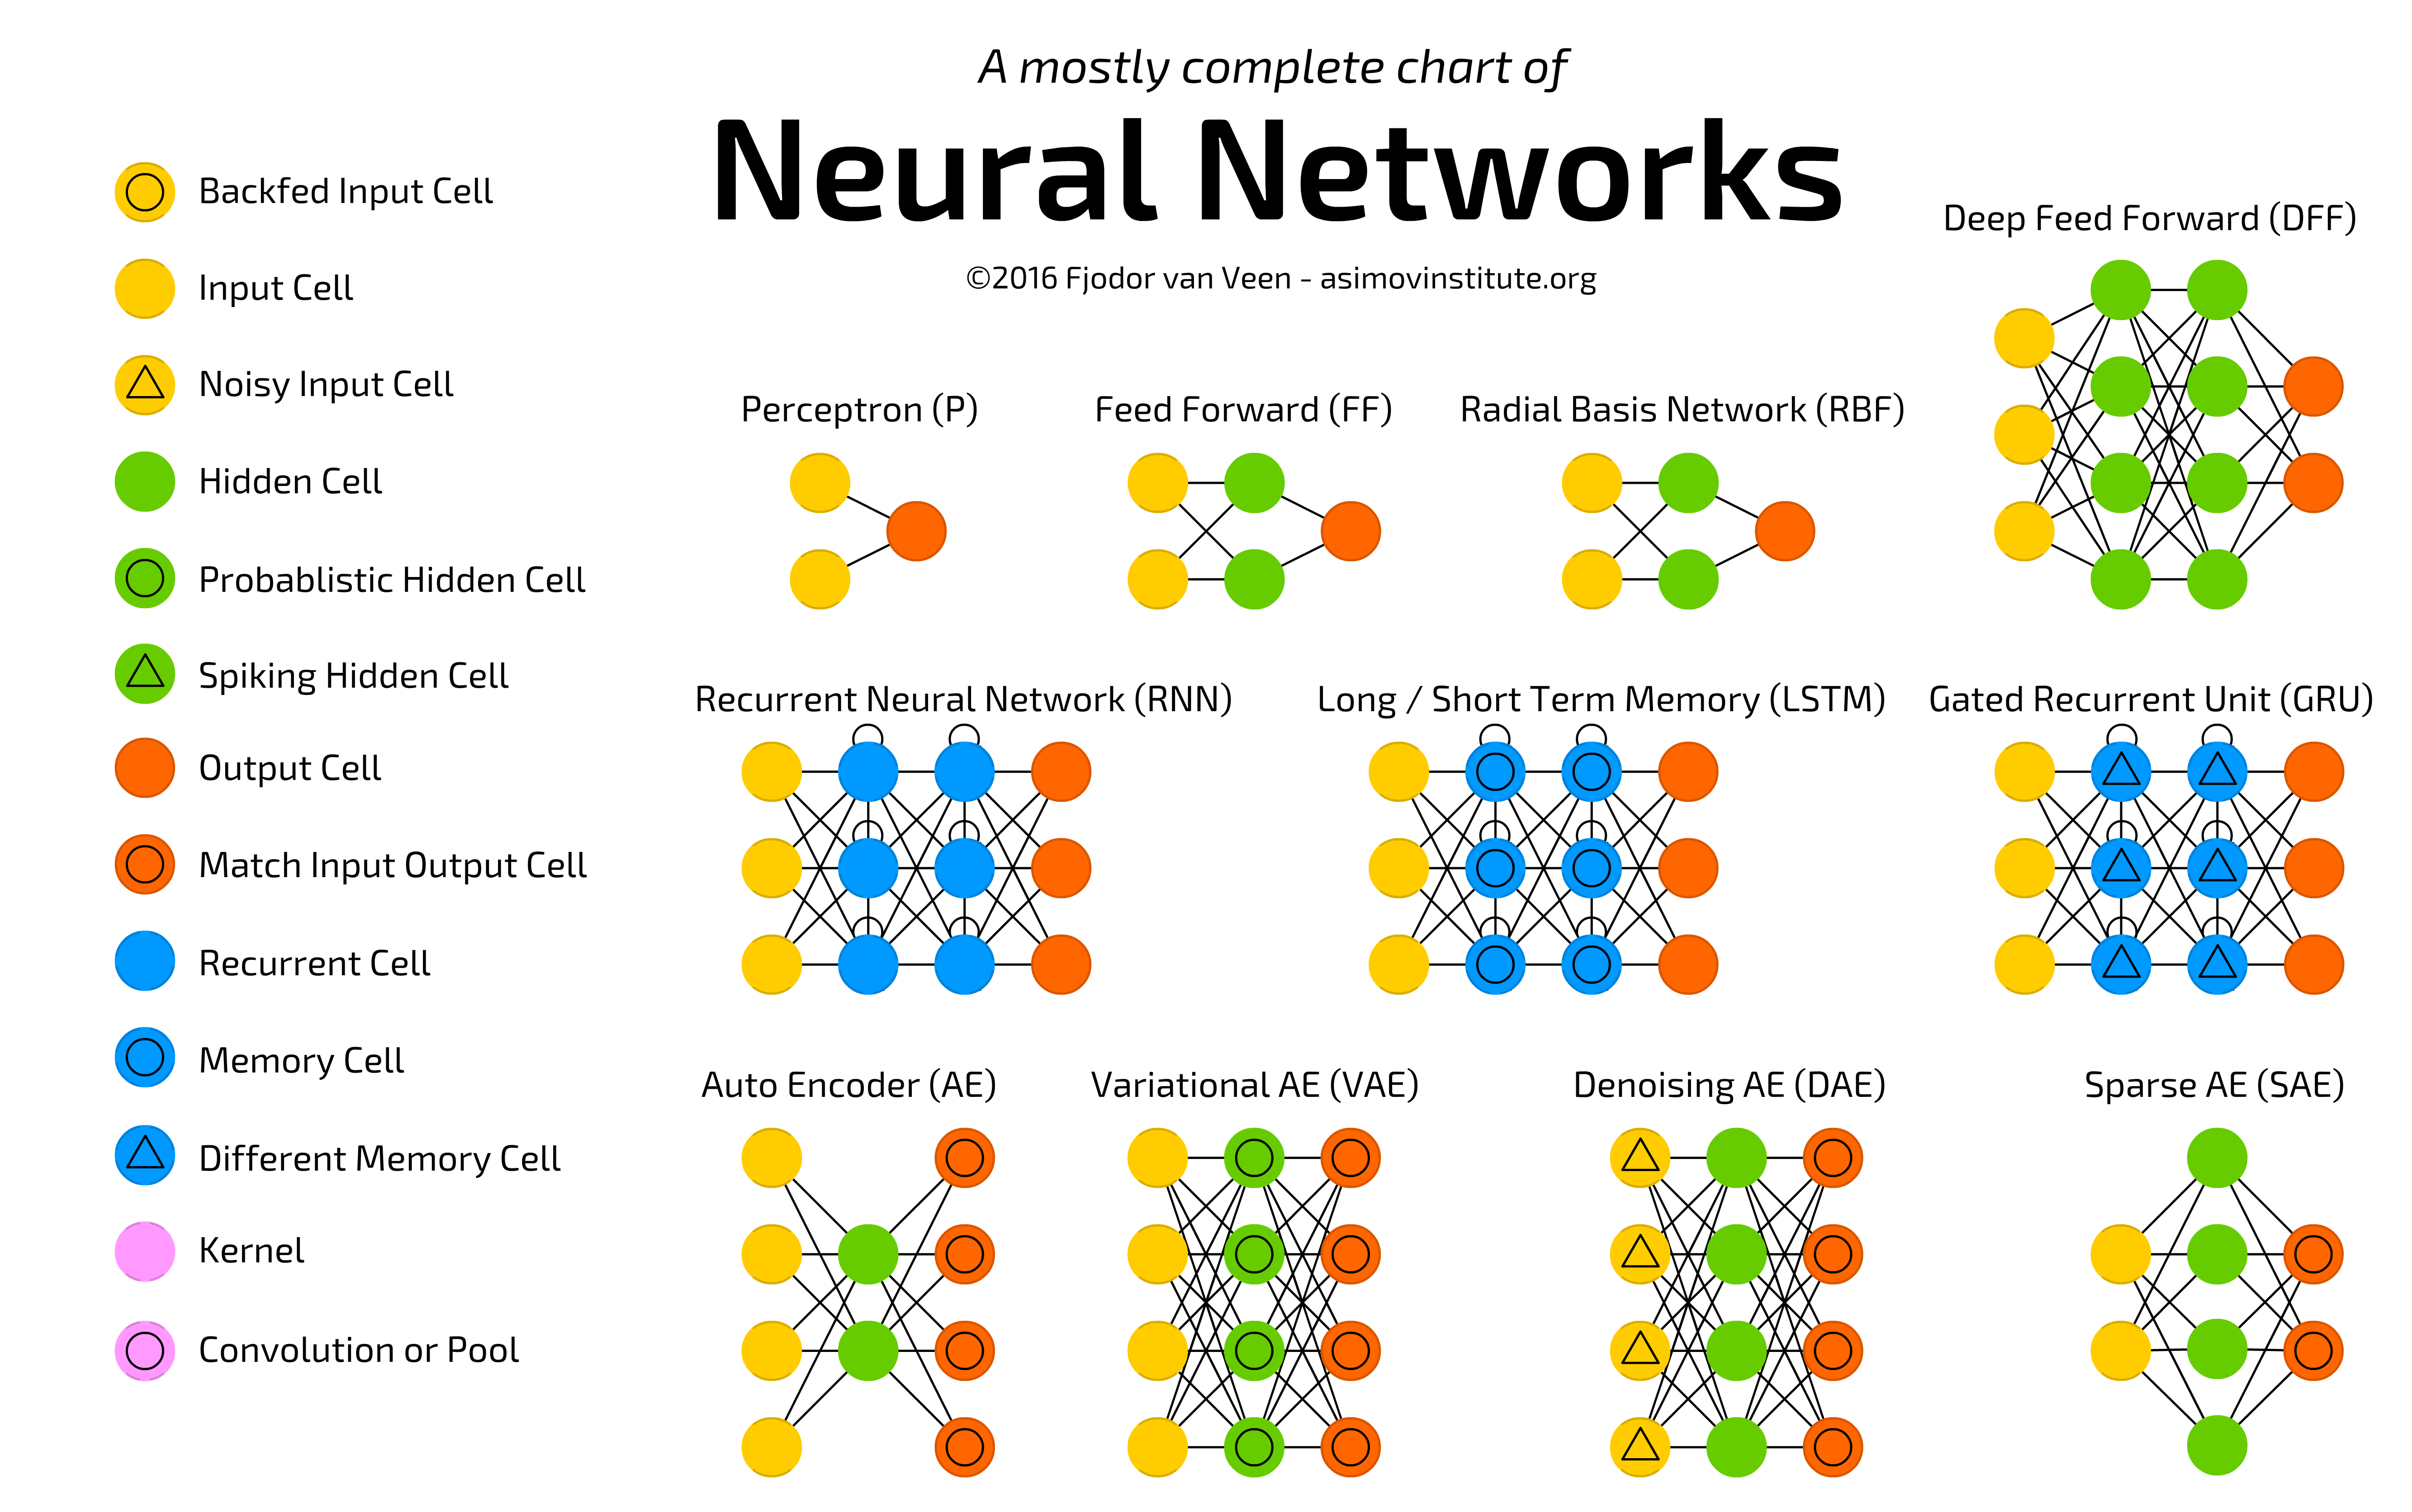
\includegraphics[width=0.8\linewidth]{networkZooPoster_1}
\end{frame}

%----------------------------------------------------------------------

\begin{frame}[c]
	\frametitle{Network architectures}
	\begin{columns}
	\column[T]{0.2\textwidth}
		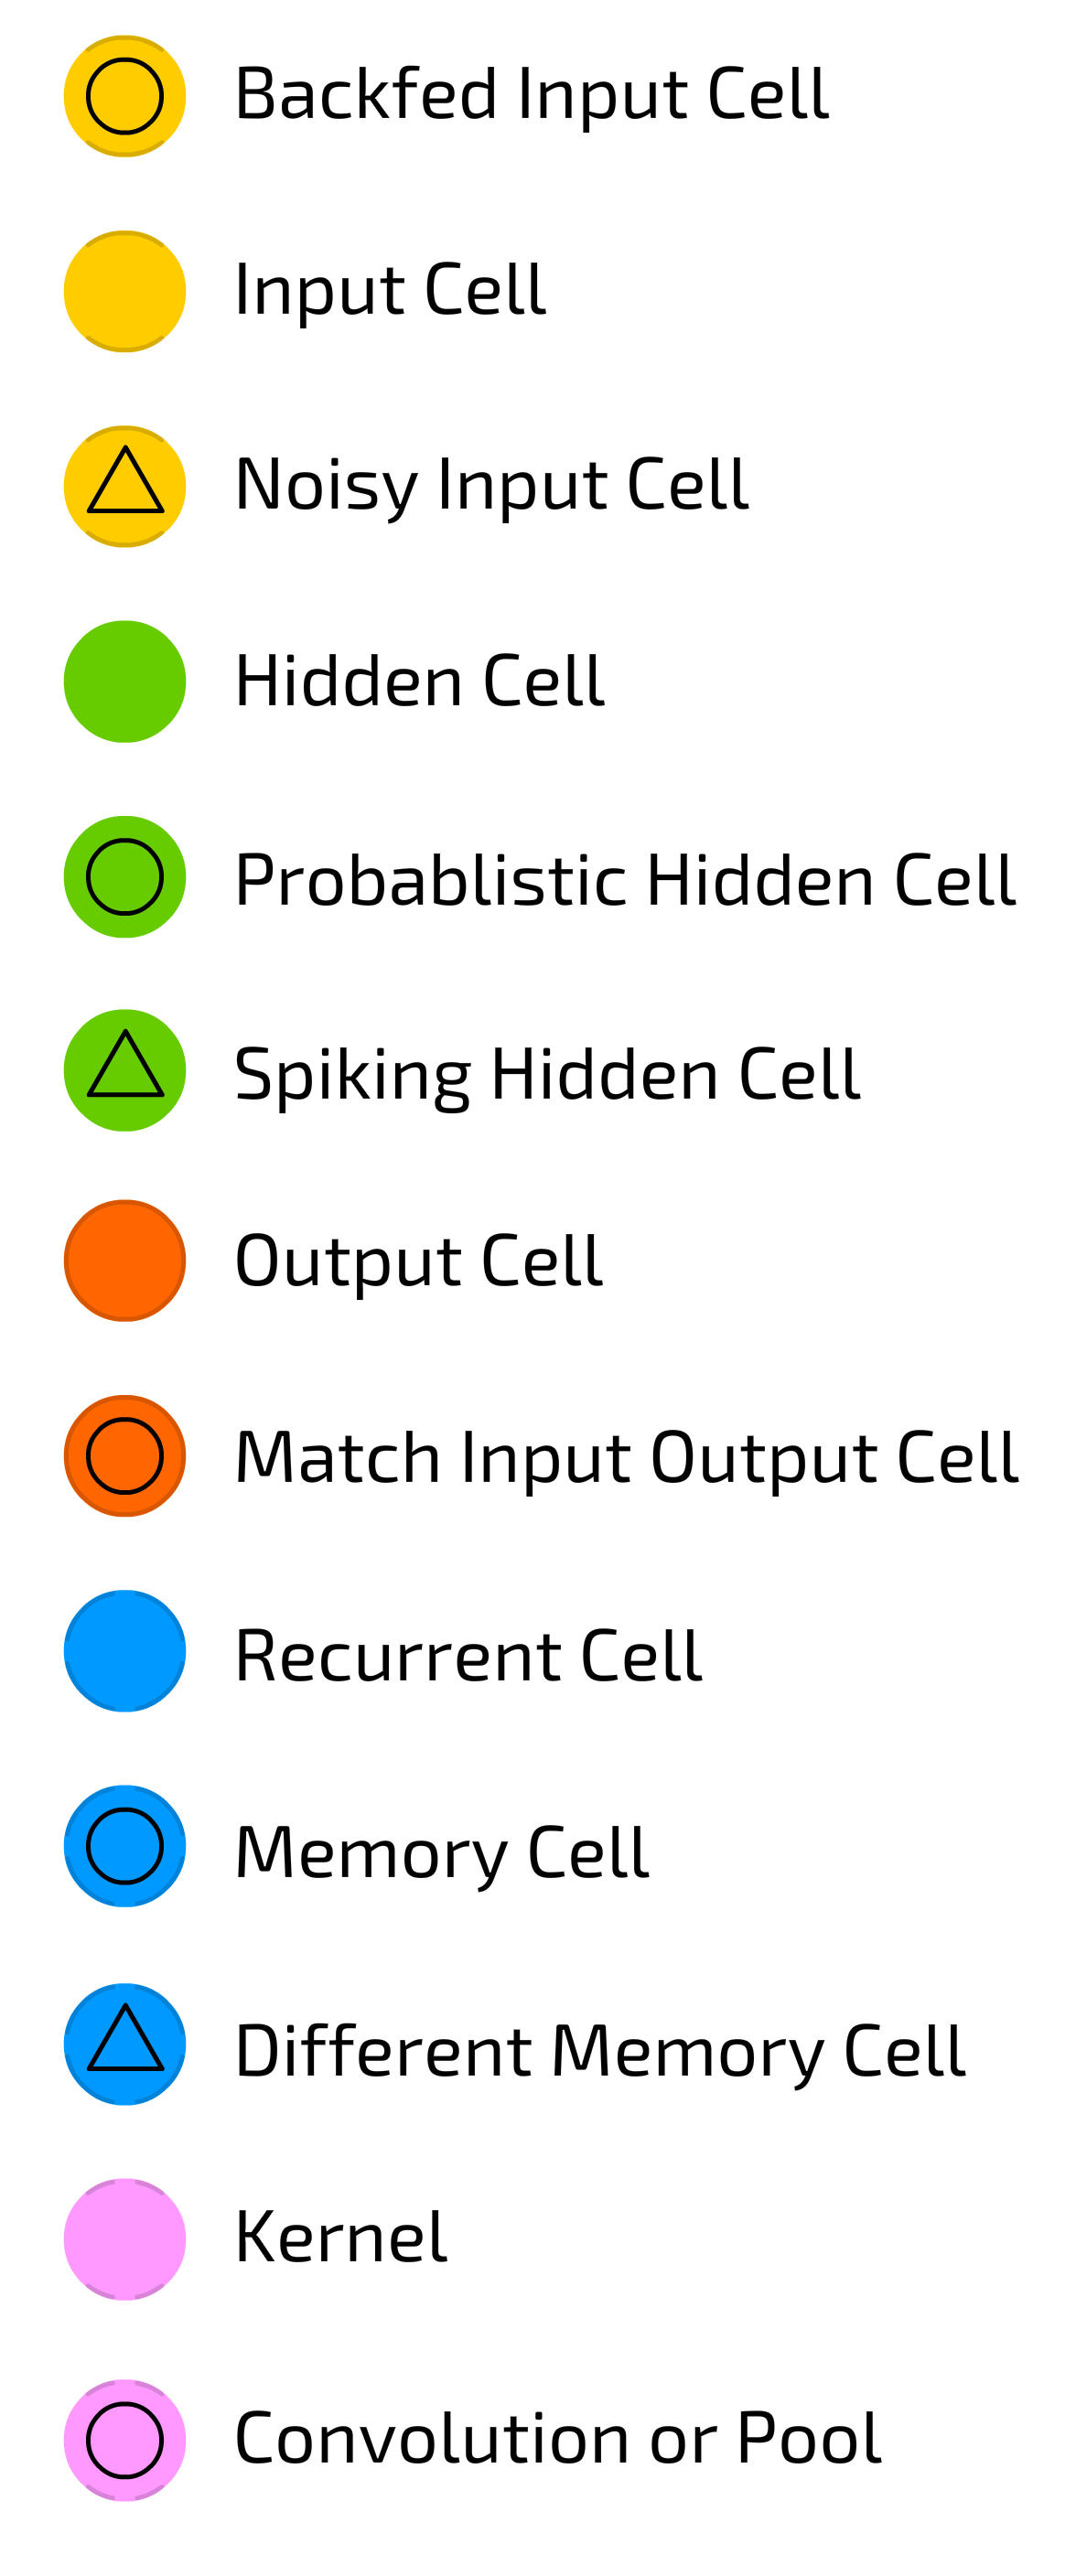
\includegraphics[width=1\linewidth]{networkZooPoster_leg}
	\column[T]{0.8\textwidth}
		\vspace{2em}
		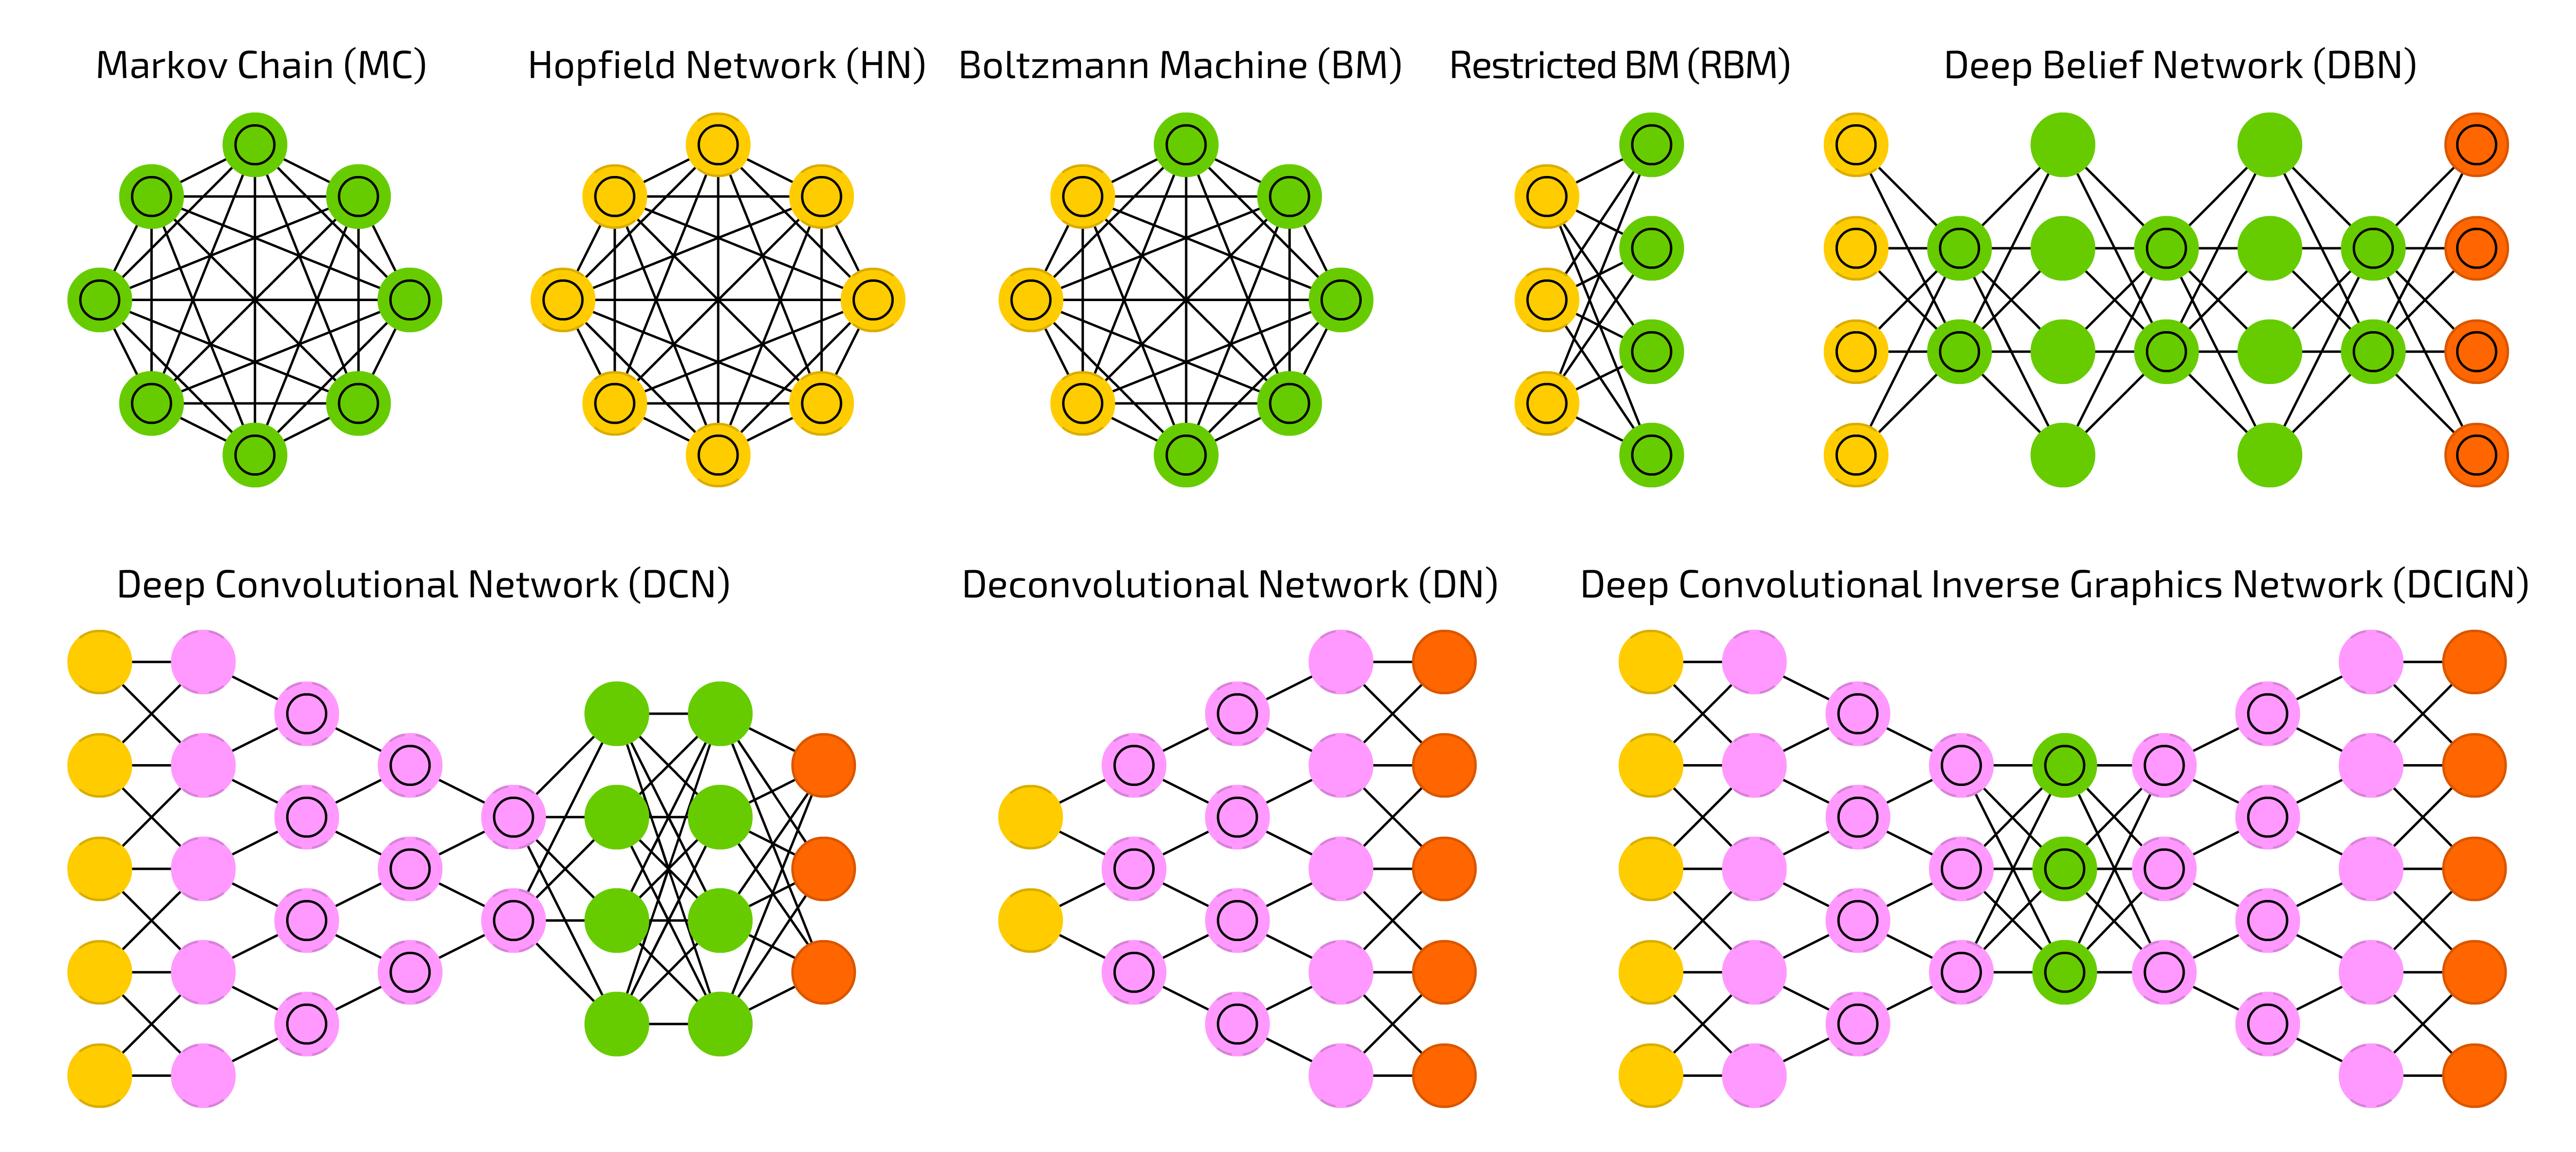
\includegraphics[width=1\linewidth]{networkZooPoster_2}
	\end{columns}
\end{frame}

%----------------------------------------------------------------------

\begin{frame}[c]
	\frametitle{Network architectures}
	\begin{columns}
		\column[T]{0.2\textwidth}
		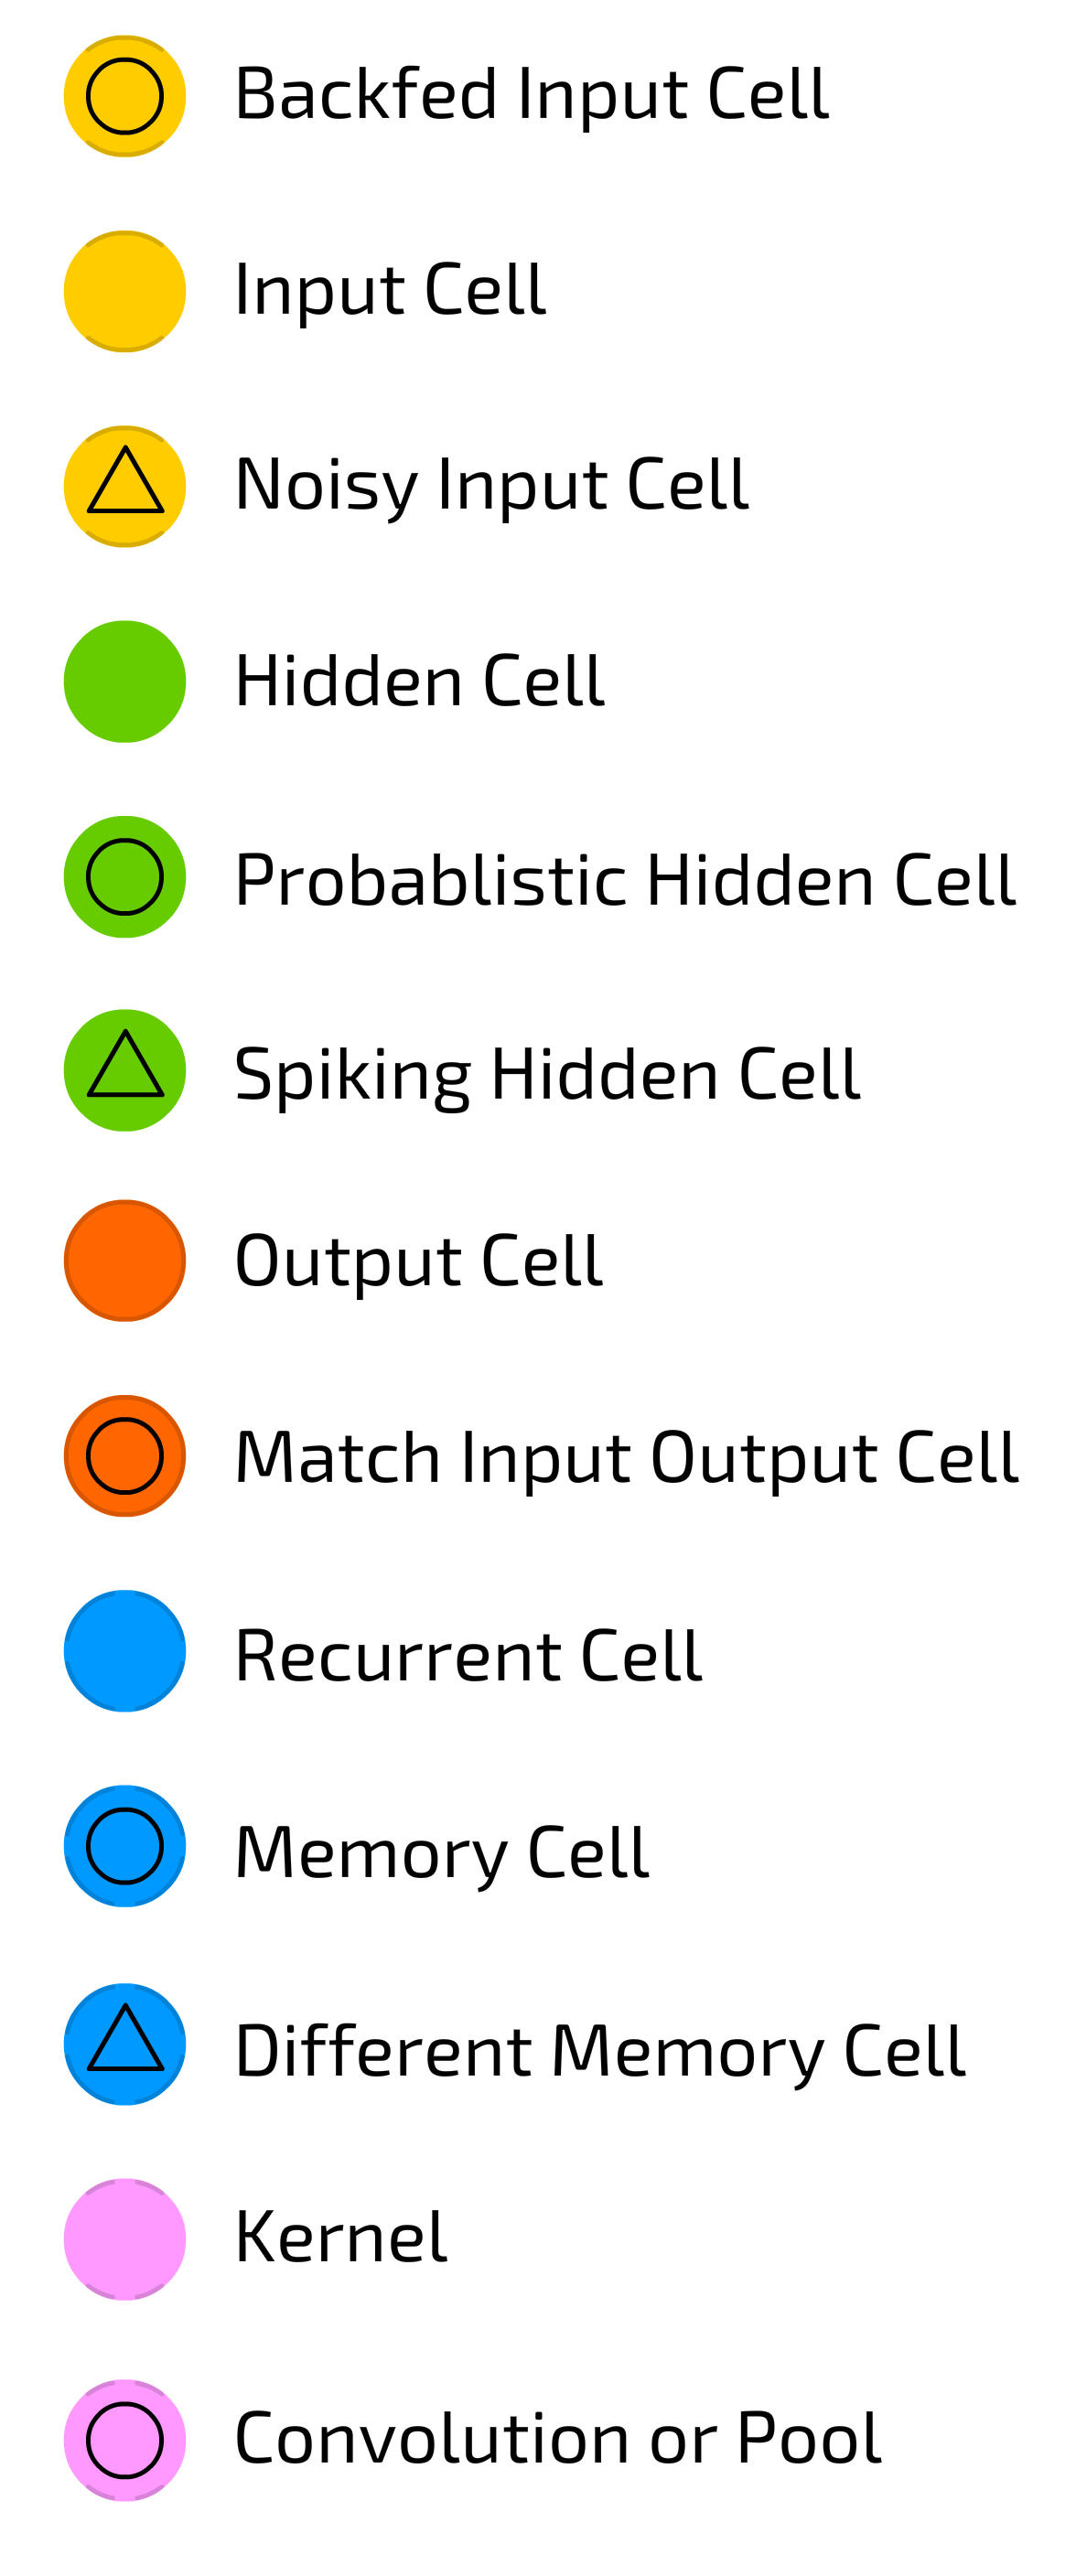
\includegraphics[width=1\linewidth]{networkZooPoster_leg}
		\column[T]{0.8\textwidth}
		\vspace{2em}
		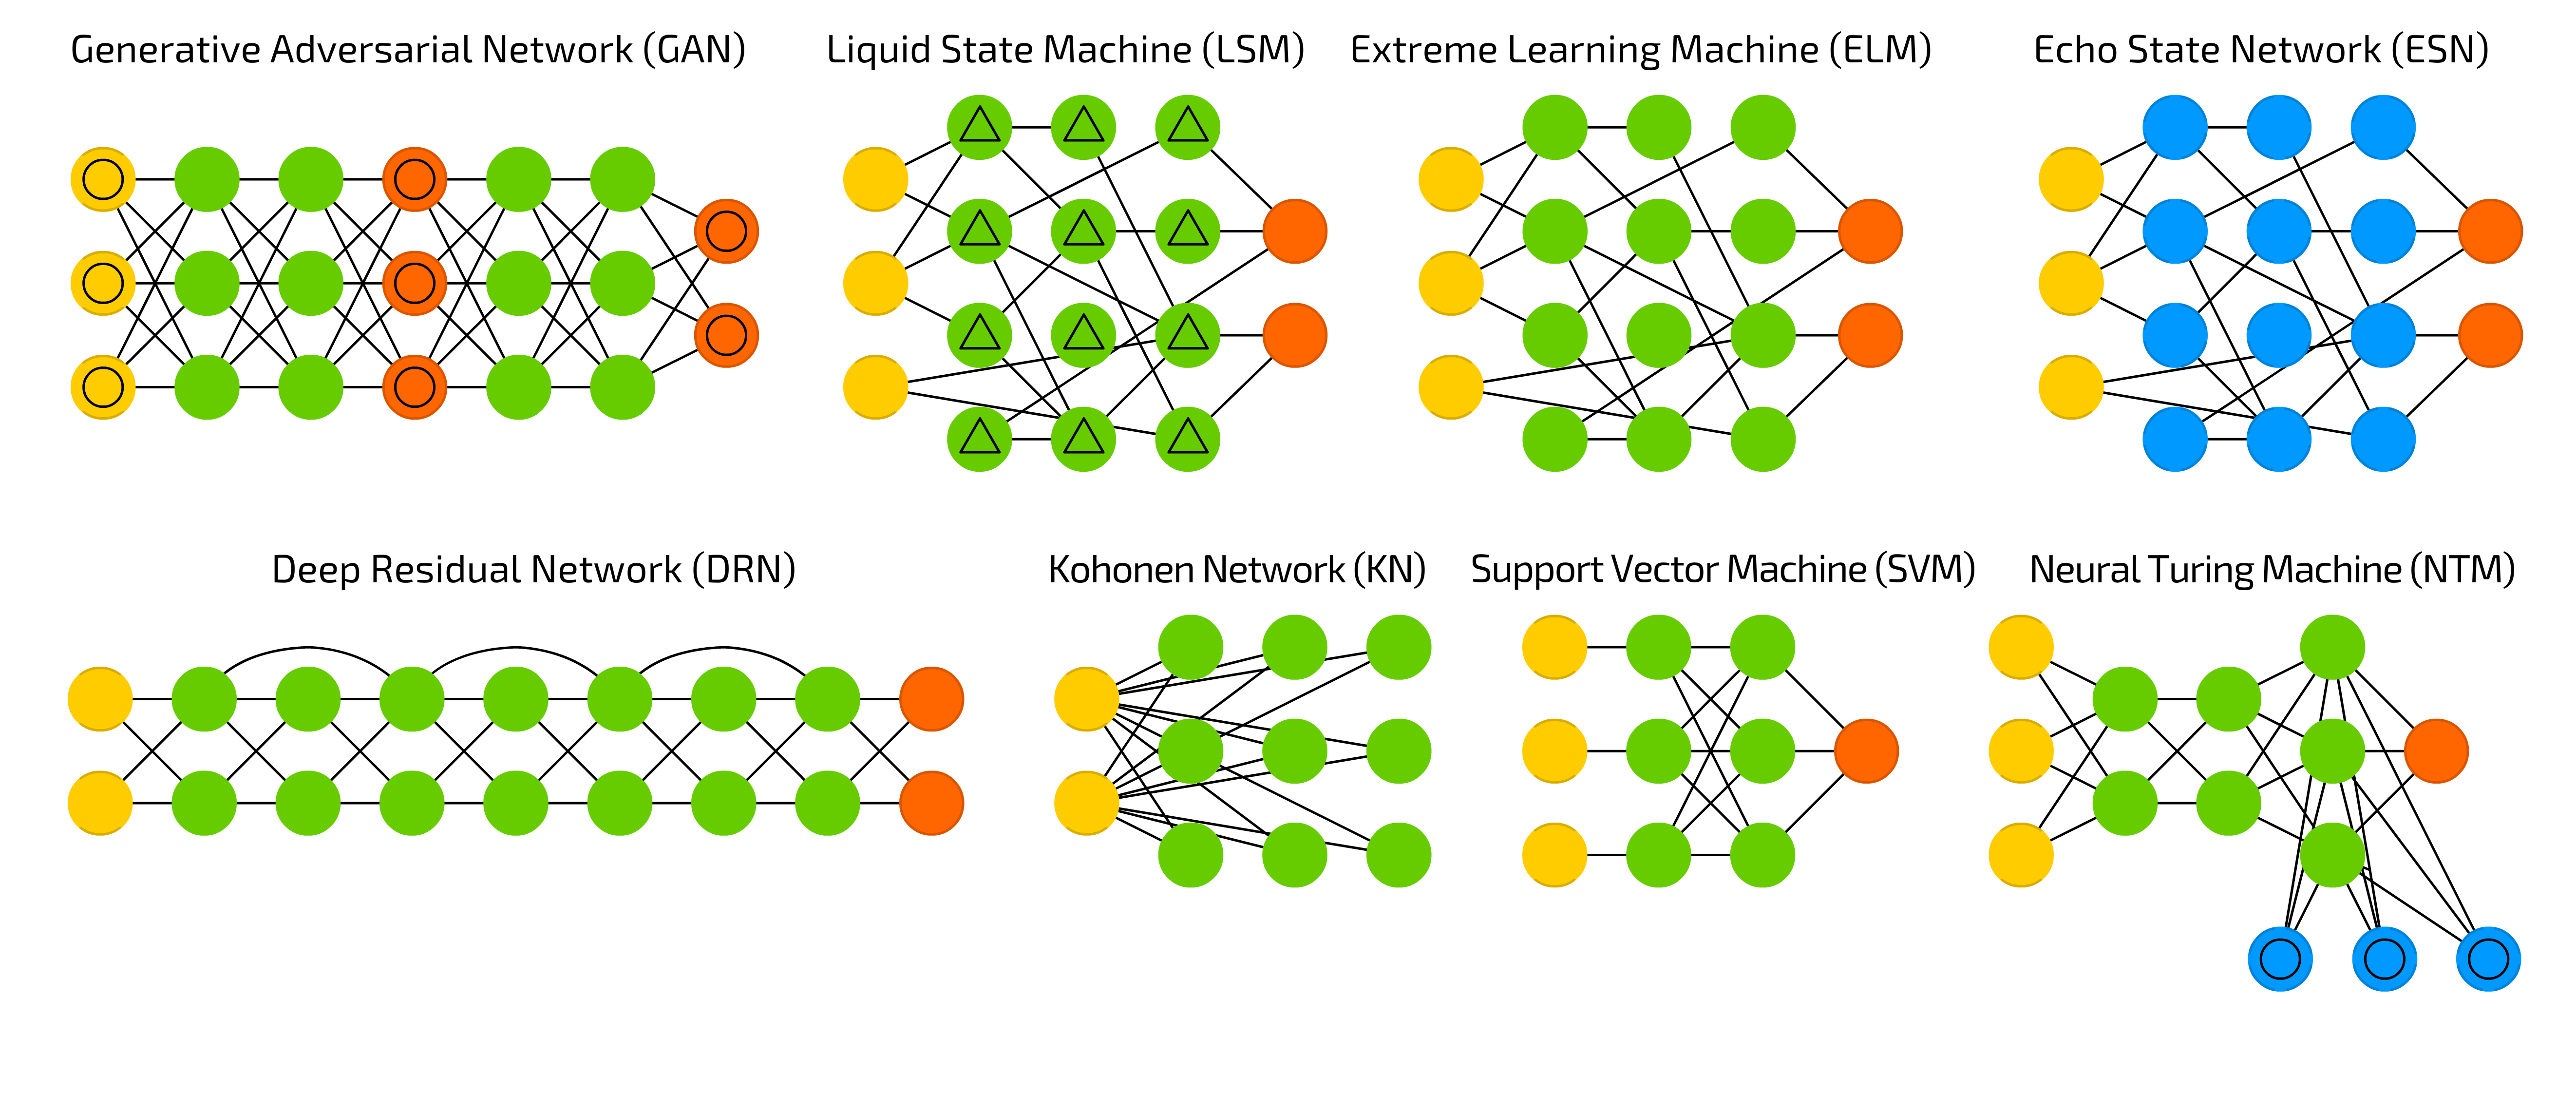
\includegraphics[width=1\linewidth]{networkZooPoster_3}
	\end{columns}
\end{frame}

%----------------------------------------------------------------------

%\backupbegin
\begin{frame}
	\frametitle{Visual pathway of the human brain}
\begin{columns}
	\column{0.5\textwidth}
	\begin{minipage}[t]{\linewidth}
		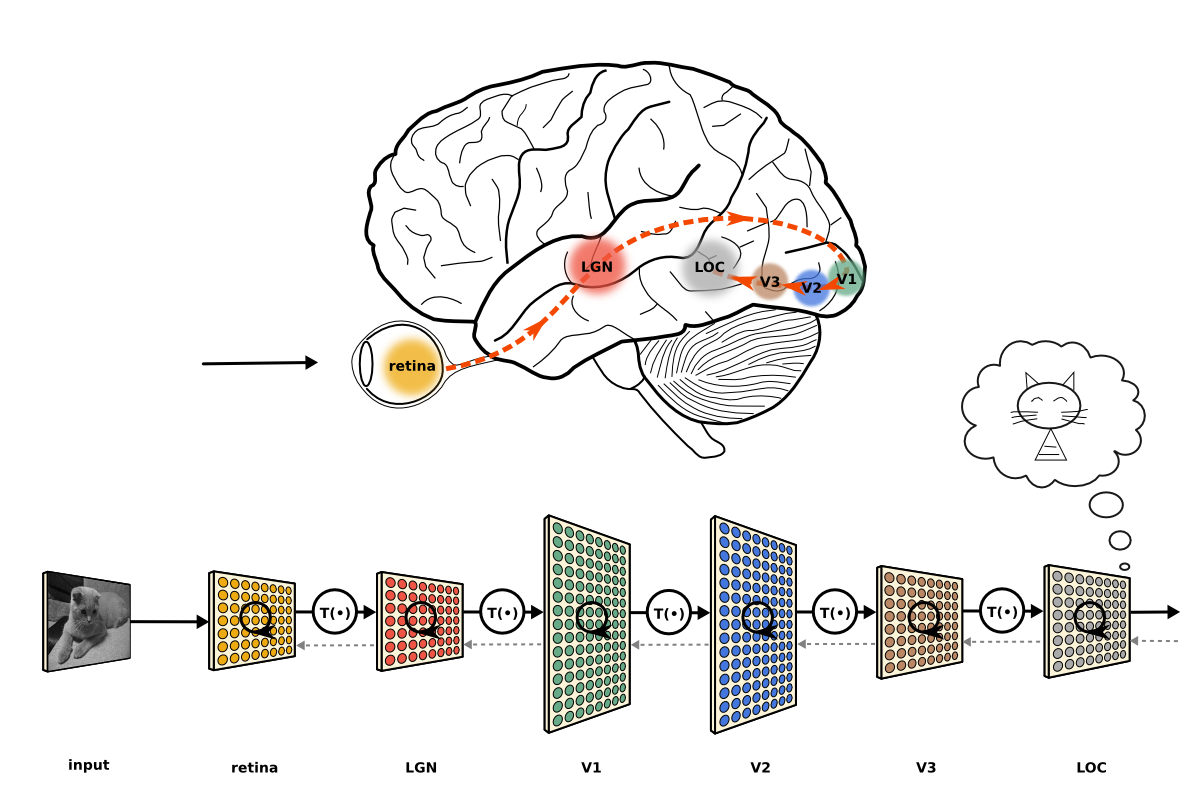
\includegraphics[width=1\linewidth]{visual_stream}
	\end{minipage}%
	\column{0.5\textwidth}
	\begin{minipage}[t]{\linewidth}
		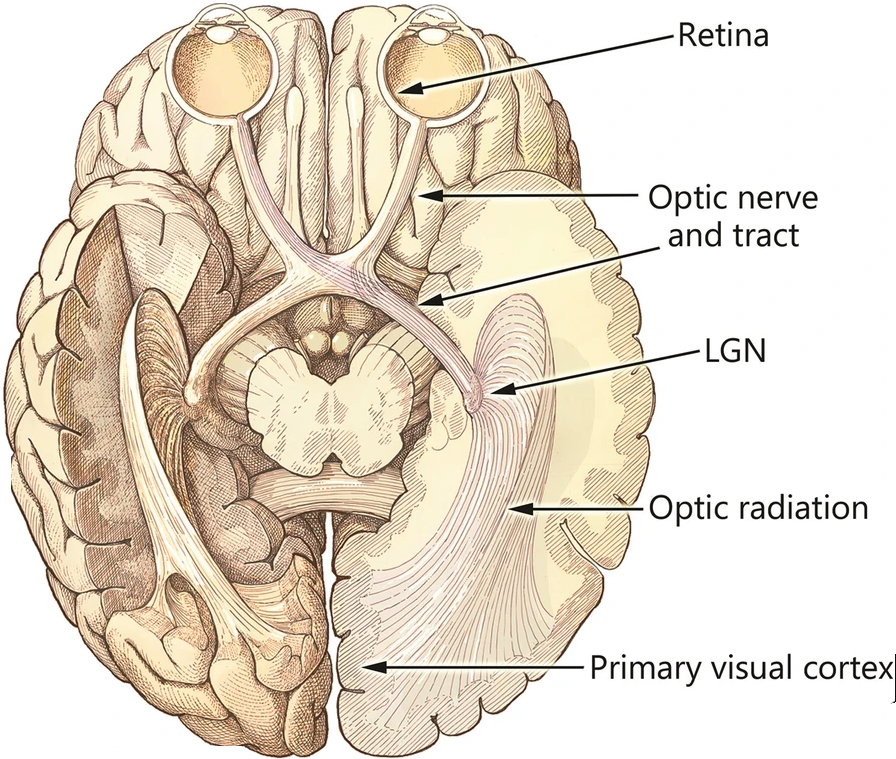
\includegraphics[width=1\linewidth]{brain_visual_pathway}
	\end{minipage}
\end{columns}
\end{frame}
%\backupend

%----------------------------------------------------------------------

\end{document}
